\newenvironment{prettylist}{
	\begin{list}{
		\footnotesize\raisebox{0pt}{\small\ding{121}}
	}{
		\setlength\topsep{2pt plus 1pt minus 1pt}
		\setlength\leftmargin{2em}
		\setlength\rightmargin{0pt}
		\setlength\itemsep{1pt plus.1pt}
		\setlength\parskip{0pt}
		\setlength\parsep{0pt}
		\setlength\itemindent{0pt}
	}
}{
	\end{list}
}
%%%%%%%%%%%%%%%%%%%%%%%%%%%%%%%%%%%%%%%%%%%%%%%
% These are the general sections to include.  %
%                                             %
% You can alter some names, but follow the    %
% suggestions in the NSF guidelines.          %
%                                             %
% If spacing is tight, play with negative     %
% vspaces w/in the text to reduce whitespace. %
%%%%%%%%%%%%%%%%%%%%%%%%%%%%%%%%%%%%%%%%%%%%%%%

%%%%%%%%%%%%%%%%%%%%%%%%%%%%%%
% Section 1: Introduction    %
%%%%%%%%%%%%%%%%%%%%%%%%%%%%%%
\section{Introduction}
\label{intro}

The proposed dissertation will systematize and address the strengths and weaknesses of emulation, dynamic analysis, modeling, and decompilation in understanding the semantics of symbol-stripped binary code.
More generally, it will provide empirically backed perspectives on the challenge of writing algorithms to analyze other algorithms under information loss conditions, drawing on four years of research in program analysis.

The first discussion centers on the domain of \emph{firmware rehosting} and Jetset, accepted to USENIX 2021, which allows codes in a specific physical domain, e.g. an ARM SoC with hardware sensors for controlling a quad-copter, to be executed and analyzed in another domain, e.g. a laptop computer.
Critically, this binary code lacks string identifiers that would aid understanding and this firmware's analysis often encounters hard problems, such as the necessity loop invariant inference.
THe primary goal of rehosting includes dynamic analysis of the a firmware image using existing offensive techniques, such as fuzzers, which cannot be carried out on the physical machine due to the possibility of damaging hardware or due to limitations on the capability of executing code.
\emph{The Jetset work led to the discovery and reproduction of a privilege escalation attack on the CMU-900's VRTX operating system.}

In discussing rehosting, the proposed dissertation will provide a greater level of technical depth and explanation on the Jetset system's approach to symbolic execution, namely, the use of symbolic execution in the inference of necessary hardware semantics for bootstrapping an emulation of a firmware image.
It will discuss the limitations of existing abstract interpretation approaches and technologies, including those used in the paper, and identify concepts essential the abstract interpretation of binary code.
The proposed dissertation will also discuss the issue of fuzzing rehosted systems and embedded systems in general, a problem that continues to see active research~\cite{zhu2022fuzzing}.
More essentially, however, Jetset introduced a specific problem: the precise modeling microarchitectural semantics and the algorithms embedded in binary code.

As a result, the present author proceeded to begin work on the precise modeling of symbol stripped binary programs, resulting in \emph{Story Beyond the Eye}, accepted to PETS 2023.
This work targeted the domain of PDF text redaction security in particular.
When compared to rehosting, the exact modeling the algorithms embedded in binary code was discovered to be more powerful for certain applications.
\emph{It was found that by exactly modeling the glyph shifting schemes of PDF document producers, novel information leaks could be ``fingerprinted'' and used to exactly de-redact the names of individuals excised from the PDF.}

The proposed dissertation will explore the extraction of algorithms for PDF document production from standard executables.
It will also detail the differences between the extraction of process traces from an embedded system like the CMU-900 and from standard executables.
Notably, it will discuss technical details involved in the dynamic analysis of embedded systems, including the necessity of trampoline code and the complexities of relocation created by the problem of binary code rewriting~\cite{wenzl2019hack}.
The utility and specifics of time-travel debugging, a form of data-flow analysis based upon stepping backwards and forwards in a program's execution, will also be made more explicit than in published results.
Reverse engineering was not the focus of \emph{Story Beyond the Eye}, despite this being the primary technical overhead, due to the novelty of the discovered attack.
Limitations, such as the fact that manual effort is required to perform the extraction of glyph shifting algorithms and only a single execution trace is recorded, will be made explicit.
This discussion provides future analysts and researchers with a blueprint for extracting glyph shifting schemes and exact reproductions of other algorithms from binary code, embedded or otherwise.

The results of both of these prior works in rehosting and algorithm extraction suggested a more general solution to several of the difficulties of binary program analysis.
In particular, there was an explicit need for a specification language and system allowing analysts to abstract arbitrary program slices into the domain of theorem provers like Z3~\cite{de2008z3}.

The dissertation therefore next addresses the InteGreat system, in submission to CAV 2023, which allows researchers to lift precise models of algorithms from embedded binary code.
The system automates several of the difficult, manual analysis steps encountered when attempting to extract algorithms from closed source binaries through an object-oriented framework for program slice abstraction (function summarization~\cite{alt2017hifrog}).
\emph{In particular, this lifting, when applied to a PLC, was useful in exactly reproducing and analyzing a code-upload attack precisely destabilizing the reactor pressure of a Eastman-Kodak chemical plant.}

Summarizing, the key contribution of the proposed dissertation is therefore a set of empirically justified statements on potential solutions to practical problems encountered when performing binary program analysis, given the empirical perspective provided by three academic works.
While not noted in this introduction, the findings also provide a well-supported argument for continued work on lifting systems and may help the uninitiated understand how computers construct meaning from symbols.
The work also provides significant insights into the concept of \emph{information loss}, both at an abstract level (e.g. when text is redacted) and at a concrete level (e.g. when a variable's name is obsfucated during compilation).

The work that composes the proposed dissertation has had immediate, broad impacts.
Jetset's core finding, an exploit for the CMU-900's operating system, resulted in direct communications with avionics manufacturers on the security of their systems.
The work on deredaction resulted in the discovery of hundreds of broken redactions, notifications of several affected parties, including the US Courts, and actions on behalf of several of these parties to prevent future information leaks. 
Moreover, the InteGreat work has already begun to affect the direction of firmware rehosting research inside the Department of Energy.

The contributions of the proposed dissertation will be:

\begin{prettylist}
\item A detailed technical explication of the techniques used to achieve significant results in three academic works, including the use of symbolic execution in firmware rehosting, full-system embedded firmware fuzzing, methodolgy for the extraction of glyph shifting algorithms for the purpose of breaking PDF text redactions, and the implementation of a framework for lifting continuous control equations from symbol-stripped binaries.
\item Empirical results attesting to the (in)effectiveness of certain solutions to the problems program analysis. These problems include path explosion during symbolic execution, the interpretation and modeling of microarchitectural semantics, and information loss during the execution, compilation, and decompilation of programs.
\item A synthesis of the concepts from otherwise disconnected, complex research works into a complete whole, providing a detailed narrative of the contemporary research landscape as it relates to systems for symbol-stripped binary code analysis and abstract interpretation of firmware images.
\end{prettylist}


%%%%%%%%%%%%%%%%%%%%%%%%%%%%%%
% Section 2: Overview        %
%%%%%%%%%%%%%%%%%%%%%%%%%%%%%%
\section{Background}
This section addresses the necessary background to understand the methodologies present in Section~\ref{sec:methods}. 
We begin by disucssing related work in firmware rehosting and the analysis of embedded systems.
Following from this, there is a brief discussion of deredaction in the context of reverse engineering---primarily, the recovery of algorithms involved in the specification of PDF documents.
Finally, we end with prior work in the verification and abstract interpretation of binary code semantics.

\subsection{Firmware Rehosting and Analysis}

The process of understanding or attacking a system like the Communication Management Unit of a Boeing 737 typically begins with the extraction of the firmware, or binary code, from hardware (flash units) storing this data, either via desoldering or via the use of wired connections~\cite{milburn2018there}.
Once this code is extracted, it is typically brought into a decompiler, such as Ghidra~\cite{eagle2020ghidra}, which lifts the binary code back into a pseudo-C representation from an intermediate representation.
This intermediate representation is typically a language with semantics that allow the decompiler to target diverse microarchitectures and allow algorithms operating on the intermediate representation to more easily perform decompilation~\cite{cifuentes1995decompilation}.
The recovered pseudo-C representation may then be reverse engineered and experimented with by researchers to better understand how the firmware functions.

However, the process of decompilation itself involves several concepts of importance to the proposed dissertations, and continues to be an active area of research~\cite{chen2019survey}.
Of these, the proposed work focuses on \emph{abstract interpretation}, introduced by Cousot and Cousot around 1977~\cite{cousot1977abstract}, a model for the static analysis of programs by the construction or approximation of fixpoints, or lifting (microarchitectural) semantics from concrete to abstract domains.

The abstract interpretation of binary programs has several equivalents, and has deeper ties into the notion of data-flow recovery and taint-tracking~\cite{schwartz2010all}.
Abstract interpretation, when applied to binary code, is often referred to as symbolic execution, for which there are several notable systems, with more popular recent examples including KLEE and angr~\cite{cadar2008klee,wang2017angr}
These systems often work by recording symbolic variants of concrete operations.
For example, the statment $(x > 5) ?\ y + 1 : x + 1$ would be concretely evaluated to 4 if $x = 3$, however, under symbolic execution, the system will record the pair $(x<=5; x=x+1),(x>5;x=y+1)$ into a symbolic state, representing the two possible execution paths.
A symbolic executor and other routines for static analysis are present in the Ghidra decompiler, in order to provide an accurate and reconfigurable reverse engineering and decompilation environment.

\textbf{Emulation and Dynamic Analysis.} One reasonable next step, beyond the decompilation of the program, is to attempt to \emph{run} the program and analyze this execution, a subdomain referred to as dynamic analysis, introduced by Ball in 1999~\cite{ball1999concept}.
For contexts in which the binary code under evaluation may be run on readily available hardware with the capability for instrumentation, it can be debugged, the execution may be traced and evaluated, or \emph{fuzzed}, inputs can be given to the system in an intelligent or random manner in order to fully evaluate the behavior of said system~\cite{li2018fuzzing}.

However, it is often \emph{not} the case that a binary program can be executed in an environment that allows for instrumentation and dynamic analysis.
Emulators, such as QEMU~\cite{bellard2005qemu}, attempt to correct for this by reproducing the context the original binary code was expecting to be emulated within, by simulating hardware interactions and by reinterpreting instructions into an microarchitecture-independent intermediate representation that may be executed on a virtual machine.

\textbf{Rehosting.} The implementation of emulators is often an arduous process, involving careful study and a precise understand of the target system and hardware context. 
The domain of \emph{firmware rehosting} attempts to automate this process, though various approaches.
Both FIE~\cite{fie} and Jetset~\cite{johnson2021jetset} attempted to use a symbolic execution to bootstrap emulators for embedded firmware: they generate symbolic constraints for algorithms the firmware uses to interact with hardware, identify execution paths leading to a desired point in the firmware's execution, and then solve the constraint sets for that path in order to recover the precise memory reads necessary to trigger that path.
Firmadyne~\cite{firmadyne} and Costin et al.~\cite{costin2014large, costin2016automated}, incontrast, attempted to just match the hardware interaction constraints of specific software, i.e. the Linux kernel and networking stacks.
Pretender~\cite{pretender2019} attempted to rehost firmware by recording the interactions between the physical hardware and the firmware. 
HALucinator~\cite{clementshalucinator} is a firmware rehosting tool that uses hueristics to locate the code belonging to the hardware abstraction layer (a vendor-provided API for interacting with the hardware) in the firmware and replace it with handlers that properly simulate the hardware interaction.
P\textsuperscript{2}IM~\cite{p2im2020} performed fuzzing to identify the correct hardware read values necessary to trigger a particular program path. 

The ultimate result of rehosting is, ideally, a system capable of executing the firmware and reproducing key system behaviors, e.g. a system that can be accurately fuzzed. 
Such a digital twin is also useful in several contexts, including the generation of digital twin systems that replicate the functioning of a complex cyberphysical system and its environment in software.
However, the domain still faces several challenges, including fidelity, firmware acquisition, static analysis for bootstrapping rehosting systems, parallelized emulation, and even after successful identification, vulnerability identification and integration of the emulation into other systems~\cite{wright2021challenges}.

The proposed disseration will shed further light on the problem of rehosting introduced by these prior works, hinted at in the methodologies of Sec.~\ref{sec:methods}, and serve to further connect the problems of rehosting to the problems of abstract interpretation and meaning-making of binary codes in the presence of lost information (e.g. hardware components, symbols).

\subsection{Deredaction and Information Leaks}
Rehosting is related to deredaction in that both problems relate to the recovery of lost information.
In the former case, the function of a system in an original, physical context, and in the latter, a removed text.
To identify these parallels and better understand information loss, the proposed dissertation next addresses the problem of \emph{deredaction}, with particular focus on PDF text.

When text is removed from a document in the classical sense, using a black marker or white-out, the width of the text is still observable given the surrounding words~\cite{egyptian}.
Considering this alone as a \emph{perfect} process on a monospaced font, the words ``cat'' and ``dog'' become indistiguishable.
However, the information loss is almost never perfect: for example, in Times New Roman, the words ``cat'' and ``dog'', if redacted, are distinguishable by their widths.
Information leaks present in redacted PDF documents were identified by Lopresti and Spitz~\cite{lopresti2004quantifying}, who developed a system for breaking redactions where the precise TTF width was known.

However, the Lopresti and Spitz work ended up failing to account for several important aspect of the problem: first that a rasterization workflow may change a PDF document's glyph positioning and physical printing may not be a pixel-perfect reproduction of the digital document, and second, that TTF glyph widths do not necessarily equate with PDF document or raster glyph widths.
Moreover, they missed an additional, severe facet of the problem: that in PDF documents, width alone was not being leaked: there are also sub-pixel sized shifts applied to non-redacted glyphs that can be \emph{dependent} on redacted glyphs' data.
This was the subject of \emph{Story Beyond the Eye}, a work narrativized by the proposed dissertation~\cite{bland2022story}.

It is useful to consider, then, cases where an information leak is not captured and cases where it is misinterpreted.
There is a wealth of literature on the improper removal of information from digital files that follows this pattern, and \emph{Story Beyond the Eye} also, understandably, only partially solves the problem.
Forrester and Irwin~\cite{forrester2005investigation} discuss nonexcising redactions and unscrubbed metadata such as the Producer field of PDF documents but do not mention glyph positioning based deredaction.
Hill et al., used hidden Markov models to recover text obscured either by mosaic pixelization or a related tactic, e.g. Gaussian Blur~\cite{hill2016effectiveness}, but fail to deredact text obscured by a single box.
While M{\"u}ller et al.~\cite{muller2021processing} discuss hidden information present in PDF documents, specifically PDF document revision information and author name metadata, but do not explicitly tackle redaction.
Other file formats may also be deredacted: Murdoch and Dornseif~\cite{murdochmisc} discuss how cropped JPEGs can preserve uncropped image information, but these works do not dicuss text redaction in particular.

Irrespective of the studied medium (PDF redaction, JPEG redaction) information left or destroyed is always a result of a communication system~\cite{ash2012information}, and in most cases this data flow is determined by a software system---by binary code interpreting binary code.
Thus the proposed dissertation will highlight a portion of \emph{Story Beyond the Eye} not discussed in the publication, the extraction of exact models of PDF text positioning algorithms from closed-source software.

\subsection{Function Summarization and Code Lifting}
\label{sec:func-summarization}

As a result of similar problems to those encountered in \emph{Story Beyond the Eye}, there is a wealth of research on the subject of \emph{function summarization} and lifting of firmware binaries, particularly within the software verification and reverse engineering communities.
The immediate form of this problem is software clone identification, which attempts to find identical program slices across binaries~\cite{zhang2021survey}, while the theoretical landscape stretches to the generation of a precise abstract interpreter from a system of logic~\cite{thakurR12}.
\emph{Function summarization} is defined as follows~\cite{interpolation}:

\emph{Let $f$ be a function, $v$ a bound on the number of unrolled loops and recursive calls, $R_{v}^{f}$ a set of tuples of computations in $f$ over $v$, $\mathbb{D}$ a domain function mapping from inputs to outputs of $f$, then $S$ s.t. $R_{v}^{f} \subseteq S \subseteq \mathbb{D}$ is a summary of $f$.}

The necessity of loop unrolling here is somewhat strict and can be replaced by inferred invariants~\cite{furia2014loop}.
\emph{Binary lifting} raises machine instructions to higher-level intermediate representations (IR) such as LLVM~\cite{anand2013compiler,di2017rev,dinaburg2014mcsema}.
The value provided by summarization and lifting is the precise association and identification of useful information within a binary program.

The final work the proposed dissertation integrates, InteGreat~\cite{bland2023integreat}, reinterprets bitvector-domain symbolic execution into the theory of uninterpreted functions to perform modular, nestable function summarization and decompilation.
It provides a specification language that allows users to abstract arbitrary program slices in symbol-stripped binary code with symbols and statements in systems of logic.

A long line of work has utilized symbolic execution to perform model extraction and subsequently verification on the extracted models.
SPIN~\cite{spin}, defined the term ``model extraction'' and applied model-checking on aero-space flight software.
Babi\'c and Hu~\cite{babic2007structural} used natural abstraction boundary identification and symbolic execution to optimize the performance of verification.
Hernandez et al.~\cite{firmusb} and~\cite{cryto-symex} used symbolic execution to extract and verify protocol models.
The same authors also noted the importance of rounding the floating-point precision error on verifying their extracted models in~\cite{precision}.
Jackson and Woodward~\cite{lightweight-oo} extracted object-oriented (OO) models from Java bytecode,~\cite{oo-model} extracted OO data models from weakly-typed source code. 
Bandera~\cite{tool-supported-program-abstraction} is a tool for user-guided extraction of finite-state automata from Java programs, however, the tool requires access to source code, and focuses on abstracting single variables rather than program slices.
While these techniques could improve InteGreat, prior work does not address the possibility of a generic language for the specification of these abstraction extraction boundaries, and does not solve the specific problems involved in stiching together uninterpreted functions as abstractions.

Ji et al.~\cite{transformation} perform backward application of extended sequent calculus rules on symbolic expression trees.
InteGreat's approach, abstraction resolution, is similar to a sequent calculus approach.
However, this work symbolically executes by sequent calculus rules and does not attempt summarization. 
Instead, the goal of the work is bisimulation and optimization of the analyzed algorithms.

The closest work to InteGreat is Currie et al.~\cite{currie2006embedded}. 
Currie et al. \emph{only} consider the problem of equivalent programs across compiler optimizations, and do not use uninterpreted functions to target \emph{decompilation}, only to check equality.
This is a stictly easier problem than the one we solve, because we address the necessity of retaining viable semantics before and after skipping a program slice (by identifying side-effects of the removed slice automatically).

The proposed dissertation will offer greater technical explanations of the core algorithms used by InteGreat and analyze the relationship between this work and that of Jetset and \emph{Story Beyond the Eye}.
It will consider how the sound substitution of a program slice's semantics via abstract interpretation, the core technical feat of InteGreat, relates to the process of information loss in transformations of digital data.
In particular, by presenting InteGreat's use of deductive specifications in the problem of abstraction, the paper will present one perspective on the nature of information loss in digital systems.

\subsection{Remaining Problems}

Because this dissertation will draw conclusions from published work and work in submission, it will only include novel experiments insofar as is necessary to justify claims made in the content of the dissertation, where existing empirical evidence will not suffice.
Unresolved domains of the proposed dissertation will include cases where the binary code under evaluation is not related to either an embedded system, a digital document, or a control equation that may be more readily abstracted than arbitrary computation.
The nature of these experiments and claims, due to realistic limitations on the grounds with which they may be justified, will be intimately related to the theoretical and real capacities of Jetset, \emph{Story Beyond the Eye}, and InteGreat.
Where appropriate the proposed dissertation will detail future work \emph{specific to the subdomain} of each work.

To provide a listing of just a few such specific future works, this includes, for example, limitations on the capabilities of existing symbolic executors to control the state space explosion encountered when attempting to interpret loops. 
It also includes difficulties in resolving pointer aliasing in symbol-stripped firmware, and lack of support within current symbolic executors for detailed support of extra-assembly semantics, such as task switching and interrupts. 
For redaction, it includes issues relating to the resolution of precise glyph shifting schemes used within printed or rasterized documents, the implementation or recovery of additional glyph shifting schemes, and the generic tracing of specific PDF production workflows.
With respect to the InteGreat work, this includes mathematical abstractions for guaranteeing the correctness of transformations between one semantic domain and an arbitrary, more abstract domain, and subsidiary issues, such as the perfect identification of a given target semantics within a symbol-stripped binary program.


%%%%%%%%%%%%%%%%%%%%%%%%%%%%%%
% Section 3: Research Plan   %
%%%%%%%%%%%%%%%%%%%%%%%%%%%%%%
\section{Research Methodology}
\label{sec:methods}

The following section introduces the methodologies and technical contributions of the Jetset, \emph{Story Beyond the Eye}, and InteGreat works.
In each subsection, an overview of the work is provided and then followed by an explanation of the specific technical contributions the dissertation will expand upon and discuss.

\subsection{Jetset}

The Jetset system uses symbolic execution to infer what behavior firmware expects from a target hardware device.
It recovers traces of the expected I/O behavior, and then generates device models for hardware peripherals in C, allowing the an analyst to boot the firmware in an emulator.
Jetset was applied to 13 firmware images, the most complex of which were a Feeder Protection Relay, the Communication Management Unit of a Boeing 737, and a Raspberry Pi.
The emulated firmware image also facilitates fuzz-testing, and a custom, architecture-independent fuzzer for QEMU, requiring no firmware modification, was used to discover a previously unknown privilege escalation vulnerability.

\subsubsection{Techniques}

The core of Jetset is composed into three parts: \emph{specification}, \emph{peripheral inference and synthesis} and \emph{search strategy}. 
The \emph{specification} fed to Jetset consists of four parts, which must be attained via alternative means:

\begin{itemize}
	\item The \textbf{binary code} of the target, which must be read out of a physical flash or extracted from the target by some other means.
	\item The \textbf{memory layout} of the target, which specifies how physical devices are mapped into the memory of the device, and is used to determine which reads and writes are key to peripheral inference.
	\item The \textbf{entry point} of the target, e.g. where execution begins. In this sense, Jetset attempts a \emph{brute force} inference of the target, by beginning inference from the absolute start of execution. This stands in contrast to InteGreat, discussed later.
	\item A \textbf{goal address} to reach within the target. Jetset explores \emph{a single} execution path to a specific firmware state, and employs a \emph{single} search strategy to get to this target. This again will stand in contrast to InteGreat.
\end{itemize}

This specification is then used to begin the process of \emph{peripheral inference and synthesis}, the former of which consists of symbolically executing the firmware to infer what values should be returned by reads from device registers.
The symbolic execution uses a taint-tracking system build on top of the QEMU TCG intermediate representation, paired with the angr constraint solver, to determine which read values are necessary to achieve a particular execution trace.
This union between taint tracking and symbolic execution was noted in~\cite{schwartz2010all}.
Jetset and the popular SymQEMU~\cite{poeplau2021symqemu}, avoid supporting hundreds of essential TCG helper methods which capture important microarchitectural semantics, such as task switching, in order to make useful theoretical discoveries.
Four attempts to elegantly address this problem culminated in the later discovery and implementation of the InteGreat system.

\begin{figure}
\centering
%\includegraphics[width=8cm]{diagrams/distance_func.png}
% Adapted from http://www.texample.net/tikz/examples/flexible-flow-chart/
\newcounter{step}
\newcommand*\step{
  \stepcounter{step}%
  \scriptsize
  \arabic{step}.
  \ttfamily
}
\begin{tikzpicture}[
  % Global options.
  >=Stealth,
  node distance=2.5ex,
  every join/.style={norm},
  every label/.style={font=\scriptsize},
  % Flow chart box styles.
  base/.style={font=\step, draw, on chain, on grid, align=center, minimum height=2ex, inner xsep=.1em, top color=black!10},
  proc/.style={base, rectangle, minimum width=4em},
  test/.style={base, diamond, aspect=2, minimum width=4em},
  % Connector styles.
  norm/.style={shorten >=1pt, ->, font=\scriptsize, pos=.3333},
  % Outline styles.
  outline/.style={draw, rectangle, densely dotted, rounded corners, inner sep=1ex},
]
% CFG for main.
{[start chain=main going below]
  \node[proc]                {call foo};
  \node[proc, join=by {"2"}] {call bar};
  \node[proc, join=by {"3"}] {call foo};
  \node[proc, join=by {"2"}] {ret};
}
\node[outline, fit=(main-begin) (main-end), label={\texttt{main} ($\mathit{length}=7$)}] {};

% CFG for foo.
{[start chain=foo going below]
  \node[proc, right=3 of main-begin] {mem[0x100] = 1};
  \node[proc, join=by {"1"}]       {eax = 2};
  \node[proc, join=by {"1"}]       {ret};
}
\node[outline, fit=(foo-begin) (foo-end), label={\texttt{foo} ($\mathit{length}=2$)}] {};

% CFG for bar.
{[start chain=bar going below]
  \node[proc, right=3.5 of foo-begin] {ebx = mem[0x200]};
  \node[test, join=by {"1"}]      {ebx == 1};
  {[start branch=then]}
  \node[proc, join=by {"\texttt{false}; 1"}] (cond) {eax = 3};
  {[continue branch=then]
    \node[proc, right=1.75 of cond,
          join=by {rounded corners,
                   to path={-|(\tikztotarget) \tikztonodes},
                   pos=.25,
                   "\texttt{true}; 1"}] {eax = 2};
  }
  \node[on chain] (dummy) {};
  \node[proc,
        join=with cond by {"1"},
        join=with bar/then-end by {
          -,
          rounded corners,
          to path={|- (dummy) \tikztonodes -| (\tikztotarget)},
          "1"}] {ret};
}
\node[outline, fit=(bar-begin) (bar/then-end) (bar-end), label={\texttt{bar} ($\mathit{length}=3$)}] {};
\end{tikzpicture}

% vim: set sw=2 sts=2 ts=8 et tw=0:

\caption{Context-sensitive distance from statement 5 (in first \texttt{foo} call) to statement 7 (of second \texttt{foo} call).}
\label{fig:distance_func}
\end{figure}

The \emph{synthesis stage} for peripherals recovers the specific model by making a call into angr's wrapper around the Z3 solver to find a concrete value that satisfies the constraints necessary to execute the desired program path.
For the purposes of finding a goal location in the firmware, Jetset naively applies just a single \emph{search strategy} to locate a target execution point, a combination of Tabu search, a variation of depth-first search guided by a distance function with a list of ``avoid'' states and a context-sensitive distance function generated by resolving the callgraph of dynamically resolved function calls during symbolic execution.
The latter is achieved by ``stitching'' the discovered call target address during the symbolic execution into the recovered control flow graph so far.
An overview of this process is given in Fig.~\ref{fig:distance_func}.

By adding the context of the child-call CFG as calls are resolved at runtime, Jetset takes into account the fact that the distance between two instructions in a program can depend on the calling context, i.e. the call-stack of the two instructions.
Because programs may modify their own callstack to perform returns to different locations, distance from the goal location is computed lazily from the actual stack during execution.
When Jetset is not able to resolve a path to the target due to indirect or runtime-calculated function pointers, it alternates between resolving branches as \emph{true} or \emph{false}, allowing it to escape from exploring the same loop resolution condition infinitely.

\subsubsection{Evaluation}

% Targets Data
\newcommand\mmio{MMIO\xspace}
\newcommand\rpitwo{Raspberry Pi 2\xspace}
\newcommand\cmutarg{CMU-900\xspace}
\newcommand\seltarg{SEL-751\xspace}

\newcommand\comma[1]{\num[group-separator={,}]{#1}}

\newcommand\rpiInfWallClockTime{6m43s}
\newcommand\rpiInfBlocksInCode{238,792}
\newcommand\rpiInfRawTotalBlocks{81194393}
\newcommand\rpiInfTotalBlocks{\num[group-separator={,}]{\rpiInfRawTotalBlocks}}
\newcommand\rpiInfTotalBlocksOnPath{81,194,393}
\newcommand\rpiInfUniqueBlocks{43,157}
\newcommand\rpiInfUniqueBlocksOnPath{43,157}
\newcommand\rpiInfWritesOnPath{84,060}
\newcommand\rpiInfReadsOnPath{83,857}
\newcommand\rpiInfWriteAddressesOnPath{40}
\newcommand\rpiInfReadAddressesOnPath{37}
\newcommand\rpiInfDevicesAccessed{6}


\newcommand\rpiSynthWallClockTime{3.16s}
\newcommand\rpiSynthSymbolicVars{1,384}
\newcommand\rpiSynthTotalConstraints{5,226}
\newcommand\rpiSynthAvgConstraints{3.78}
\newcommand\rpiSynthMedConstraints{4}
\newcommand\rpiSynthMaxConstraints{30}
\newcommand\rpiSynthAvgTraceLen{37.4}
\newcommand\rpiSynthMedTraceLen{1}
\newcommand\rpiSynthMaxTraceLen{1076}


\newcommand\rpiEmuWallClockTime{8s}

\newcommand\rpiEmuRawTotalBlocks{81454594}
\newcommand\printpercent[2]{\FPeval\result{round(#1*100/#2,1)}\result\%}
\newcommand\printpercentmore[2]{\FPeval\result{round(#1/#2-1,1)}\result\%}
\newcommand\rpiRawEmuTotalBlocks{43227}
\newcommand\rpiEmuTotalBlocks{\num[group-separator={,}]{\rpiEmuRawTotalBlocks}}
\newcommand\rpiEmuPercBlocksMore{\printpercentmore{\rpiEmuRawTotalBlocks}{\rpiInfRawTotalBlocks}}

\newcommand\rpiEmuUniqueBlocks{43,255}
\newcommand\rpiEmuWritesOnPath{83,915}
\newcommand\rpiEmuReadsFromTrace{83,857}
\newcommand\rpiEmuReadsBeyondTrace{0}
\newcommand\rpiEmuWriteAddresses{43}
\newcommand\rpiEmuReadAddresses{27}
\newcommand\rpiEmuDevicesAccessed{6}
                                                                           
\newcommand\bbxmInfWallClockTime{5m15s}
\newcommand\bbxmInfBlocksInCode{872}
\newcommand\bbxmInfTotalBlocks{20,198,824}
\newcommand\bbxmInfTotalBlocksOnPath{20,198,824}
\newcommand\bbxmInfUniqueBlocks{484}
\newcommand\bbxmInfUniqueBlocksOnPath{484}
\newcommand\bbxmInfWritesOnPath{938}
\newcommand\bbxmInfReadsOnPath{3,633}
\newcommand\bbxmInfWriteAddressesOnPath{244}
\newcommand\bbxmInfReadAddressesOnPath{61}
\newcommand\bbxmInfDevicesAccessed{11}


\newcommand\bbxmSynthWallClockTime{5.64s}
\newcommand\bbxmSynthSymbolicVars{\bbxmInfReadsOnPath}
\newcommand\bbxmSynthTotalConstraints{8,353}
\newcommand\bbxmSynthAvgConstraints{2.30}
\newcommand\bbxmSynthMedConstraints{2}
\newcommand\bbxmSynthMaxConstraints{74}
\newcommand\bbxmSynthAvgTraceLen{59.56}
\newcommand\bbxmSynthMedTraceLen{3}
\newcommand\bbxmSynthMaxTraceLen{2,770}

\newcommand\bbxmEmuWallClockTime{101ms}
\newcommand\bbxmEmuTotalBlocks{20,198,656}
\newcommand\bbxmEmuUniqueBlocks{483}
\newcommand\bbxmEmuWritesOnPath{938}
\newcommand\bbxmEmuReadsFromTrace{3,633}
\newcommand\bbxmEmuReadsBeyondTrace{0}
\newcommand\bbxmEmuWriteAddresses{244}
\newcommand\bbxmEmuReadAddresses{61}
\newcommand\bbxmEmuDevicesAccessed{11}
                                                                           
\newcommand\cmuInfWallClockTime{5m20s}
\newcommand\cmuInfBlocksInCode{55,016}
\newcommand\cmuInfTotalBlocks{53,143,508}
\newcommand\cmuInfRawTotalBlocksOnPath{27517932}
\newcommand\cmuInfTotalBlocksOnPath{\num[group-separator={,}]{\cmuInfRawTotalBlocksOnPath}}
\newcommand\cmuInfUniqueBlocks{776}
\newcommand\cmuInfUniqueBlocksOnPath{731}
\newcommand\cmuInfWritesOnPath{1,308}
\newcommand\cmuInfReadsOnPath{242}
\newcommand\cmuInfWriteAddressesOnPath{13}
\newcommand\cmuInfReadAddressesOnPath{5}
\newcommand\cmuInfDevicesAccessed{5}


\newcommand\cmuSynthWallClockTime{0.018s}
\newcommand\cmuSynthSymbolicVars{\cmuInfReadsOnPath}
\newcommand\cmuSynthTotalConstraints{756}
\newcommand\cmuSynthAvgConstraints{3.12}
\newcommand\cmuSynthMedConstraints{3}
\newcommand\cmuSynthMaxConstraints{11}
\newcommand\cmuSynthAvgTraceLen{48.4}
\newcommand\cmuSynthMedTraceLen{5}
\newcommand\cmuSynthMaxTraceLen{215}

\newcommand\cmuEmuWallClockTime{289ms}
\newcommand\cmuEmuRawTotalBlocks{27519080}
\newcommand\cmuEmuTotalBlocks{\num[group-separator={,}]{\cmuEmuRawTotalBlocks}}
\newcommand\cmuEmuUniqueBlocks{731}
\newcommand\cmuEmuWritesOnPath{1,882}
\newcommand\cmuEmuReadsFromTrace{242}
\newcommand\cmuEmuReadsBeyondTrace{0}
\newcommand\cmuEmuWriteAddresses{13}
\newcommand\cmuEmuReadAddresses{5}
\newcommand\cmuEmuDevicesAccessed{5}
                                                                           
\newcommand\selInfWallClockTime{2h34m51s}
\newcommand\selInfBlocksInCode{141,750}
\newcommand\selInfTotalBlocks{3,351,484,857}
\newcommand\selInfTotalBlocksOnPath{3,351,484,857}
\newcommand\selInfUniqueBlocks{11,364}
\newcommand\selInfUniqueBlocksOnPath{11,364}
\newcommand\selInfWritesOnPath{32,480}
\newcommand\selInfReadsOnPath{704}
\newcommand\selInfWriteAddressesOnPath{68}
\newcommand\selInfReadAddressesOnPath{26}
\newcommand\selInfDevicesAccessed{5}


\newcommand\selSynthWallClockTime{5.61s}
\newcommand\selSynthSymbolicVars{\selInfReadsOnPath}
\newcommand\selSynthTotalConstraints{11,142}
\newcommand\selSynthAvgConstraints{15.83}
\newcommand\selSynthMedConstraints{5}
\newcommand\selSynthMaxConstraints{1279}
\newcommand\selSynthAvgTraceLen{27.08}
\newcommand\selSynthMedTraceLen{2}
\newcommand\selSynthMaxTraceLen{343}

\newcommand\selEmuWallClockTime{1m1s}
\newcommand\selEmuTotalBlocks{3,351,502,947}
\newcommand\selEmuUniqueBlocks{11,364}
\newcommand\selEmuWritesOnPath{32,480}
\newcommand\selEmuReadsFromTrace{704}
\newcommand\selEmuReadsBeyondTrace{0}
\newcommand\selEmuWriteAddresses{68}
\newcommand\selEmuReadAddresses{26}
\newcommand\selEmuDevicesAccessed{5}

% Misc
\newcommand\numCmuVulns{1}
\newcommand\dtbFileDevices{28}
\newcommand\rpiDistinctSyscalls{1,571,576}

\newcommand\numXloadRegns{200}
\newcommand\numXloadSynDevs{TODO}
\newcommand\numHrsXload{TODO}
\newcommand\numLinxBrch{TODO}
\newcommand\numLinxIndrJumps{TODO}

% RPI Eval Data
\newcommand\rpiSyscallsIssued{}
\newcommand\rpiRawNumPathsDiscovered{123198}
\newcommand\rpiNumPathsDiscovered{\num[group-separator={,}]{\rpiRawNumPathsDiscovered}}
\newcommand\rpiHexDumpDiffsNum{51,592}
\newcommand\rpiHexDumpDiffsPerc{41.9\%}
\newcommand\rpiRawNumDeaths{51638}
\newcommand\rpiNumDeaths{\num[group-separator={,}]{\rpiRawNumDeaths}}
\newcommand\subtract[2]{\FPeval\result{round(#1-#2,0)}\comma{\result}}
\newcommand\rpiNumReturns{\subtract{\rpiRawNumPathsDiscovered}{\rpiRawNumDeaths}}
\newcommand\rpiPhysicalTestCases{14,661}

% CMU Eval Data
\newcommand\cmuRawNumPathsDiscovered{2963}
\newcommand\cmuNumPathsDiscovered{\comma{\cmuRawNumPathsDiscovered}}
\newcommand\cmuHoursFuzzed{200}
\newcommand\cmuRawExactOutputMatches{2884}
\newcommand\cmuExactOutputMatches{\comma{\cmuRawExactOutputMatches}}
\newcommand\cmuNearExactOutputMatches{36}
\newcommand\cmuNonExactOutputMatches{43}
\newcommand\cmuDifferenceInBlocksExecuted{\subtract{\cmuEmuRawTotalBlocks}{\cmuInfRawTotalBlocksOnPath}}

\newcommand\cmuPercentNonExactOutputToPaths{\printpercent{\cmuNonExactOutputMatches}{\cmuRawNumPathsDiscovered}}
\newcommand\cmuPercentNearOutputToPaths{\printpercent{\cmuNearExactOutputMatches}{\cmuRawNumPathsDiscovered}}
\newcommand\cmuPercentExactOutputToPaths{\printpercent{\cmuRawExactOutputMatches}{\cmuRawNumPathsDiscovered}}

\newcommand\bbxmDatasheetPeris{35}


\begin{table*}
\small
\centering
\caption{Evaluation targets and summary statistics.}
\label{tab:targets}
\begin{tabular}{@{}lllrrr@{}}
  \toprule
  \quad                       &                                                     & \multicolumn{2}{r}{\textbf{\rpitwo}}      & \textbf{\cmutarg}            & \textbf{\seltarg}            \\
  \midrule
  \multicolumn{2}{@{}l}{CPU/SoC} & \multicolumn{2}{r}{Broadcom BCM2836 (ARM)}       & AMD~Am486 (i386)             & NXP~MCF54455 (ColdFire)                                   \\
  \multicolumn{2}{@{}l}{OS/SW}   & \multicolumn{2}{r}{Linux 4.19.y}                 & VRTX-32                      & G5.1.5.0                                                  \\
  \multicolumn{3}{@{}l}{\emph{Peripheral inference}}                                                                                                                                                                        \\
                              & \multicolumn{2}{l}{Wall-clock time}                 & \rpiInfWallClockTime                        & \cmuInfWallClockTime        & \selInfWallClockTime        \\
                              & \multicolumn{2}{l}{Blocks in code base}             & \rpiInfBlocksInCode                         & \cmuInfBlocksInCode         & \selInfBlocksInCode         \\
                              & \multicolumn{2}{l}{Total blocks executed}           & \rpiInfTotalBlocks                          & \cmuInfTotalBlocks          & \selInfTotalBlocks          \\
                              & \multicolumn{2}{l}{Blocks executed on path}         & \rpiInfTotalBlocksOnPath                    & \cmuInfTotalBlocksOnPath    & \selInfTotalBlocksOnPath    \\
                              & \multicolumn{2}{l}{Unique blocks executed}          & \rpiInfUniqueBlocks                         & \cmuInfUniqueBlocks         & \selInfUniqueBlocks         \\
                              & \multicolumn{2}{l}{Unique blocks executed on path}  & \rpiInfUniqueBlocksOnPath                   & \cmuInfUniqueBlocksOnPath   & \selInfUniqueBlocksOnPath   \\
                              & \multicolumn{2}{l}{\mmio\ writes (ignored) on path} & \rpiInfWritesOnPath                         & \cmuInfWritesOnPath         & \selInfWritesOnPath         \\
                              & \multicolumn{2}{l}{\mmio\ reads (symbolic) on path} & \rpiInfReadsOnPath                          & \cmuInfReadsOnPath          & \selInfReadsOnPath          \\
                              & \multicolumn{2}{l}{\mmio\ write addresses on path}  & \rpiInfWriteAddressesOnPath                 & \cmuInfWriteAddressesOnPath & \selInfWriteAddressesOnPath \\
                              & \multicolumn{2}{l}{\mmio\ read addresses on path}   & \rpiInfReadAddressesOnPath                  & \cmuInfReadAddressesOnPath  & \selInfReadAddressesOnPath  \\
                              & \multicolumn{2}{l}{Devices accessed}                & \rpiInfDevicesAccessed                      & \cmuInfDevicesAccessed      & \selInfDevicesAccessed      \\
  % Fix to be just the peripherals
  \multicolumn{3}{@{}l}{\emph{Peripheral synthesis}}                                                                                                                                                                            \\
                              & \multicolumn{2}{l}{Wall-clock time}                 & \rpiSynthWallClockTime                      & \cmuSynthWallClockTime      & \selSynthWallClockTime      \\
                              & \multicolumn{2}{l}{Total Symbolic Variables}        & \rpiSynthSymbolicVars                       & \cmuSynthSymbolicVars       & \selSynthSymbolicVars       \\
                              & \multicolumn{2}{l}{Total Constraints}               & \rpiSynthTotalConstraints                   & \cmuSynthTotalConstraints   & \selSynthTotalConstraints   \\
                              & \multicolumn{2}{l}{Constraints per variable}   & \rpiSynthAvgConstraints                     & \cmuSynthAvgConstraints     & \selSynthAvgConstraints     \\
%                              & \multicolumn{2}{l}{Med. constraints per variable}   & \rpiSynthMedConstraints                     & \cmuSynthMedConstraints     & \selSynthMedConstraints     \\
%                              & \multicolumn{2}{l}{Max. constraints per variable}   & \rpiSynthMaxConstraints                     & \cmuSynthMaxConstraints     & \selSynthMaxConstraints     \\
                              & \multicolumn{2}{l}{Average trace length}               & \rpiSynthAvgTraceLen                        & \cmuSynthAvgTraceLen        & \selSynthAvgTraceLen        \\
                              & \multicolumn{2}{l}{Median trace length}               & \rpiSynthMedTraceLen                        & \cmuSynthMedTraceLen        & \selSynthMedTraceLen        \\
                              & \multicolumn{2}{l}{Maximum trace length}               & \rpiSynthMaxTraceLen                        & \cmuSynthMaxTraceLen        & \selSynthMaxTraceLen        \\
  \multicolumn{3}{@{}l}{\emph{Emulator execution to goal}}                                                                                                                                                                      \\
                              & \multicolumn{2}{l}{Wall-clock time}                 & \rpiEmuWallClockTime                        & \cmuEmuWallClockTime        & \selEmuWallClockTime        \\
                              & \multicolumn{2}{l}{Total blocks executed}           & \rpiEmuTotalBlocks                          & \cmuEmuTotalBlocks          & \selEmuTotalBlocks          \\
                              & \multicolumn{2}{l}{Unique blocks executed}          & \rpiEmuUniqueBlocks                         & \cmuEmuUniqueBlocks         & \selEmuUniqueBlocks         \\
                              & \multicolumn{2}{l}{\mmio\ writes (ignored)}         & \rpiEmuWritesOnPath                         & \cmuEmuWritesOnPath         & \selEmuWritesOnPath         \\
                              & \multicolumn{2}{l}{\mmio\ reads}                    & \rpiEmuReadsFromTrace                       & \cmuEmuReadsFromTrace       & \selEmuReadsFromTrace       \\
                              & \multicolumn{2}{l}{\mmio\ write addresses}          & \rpiEmuWriteAddresses                       & \cmuEmuWriteAddresses       & \selEmuWriteAddresses       \\
                              & \multicolumn{2}{l}{\mmio\ read addresses}           & \rpiEmuReadAddresses                        & \cmuEmuReadAddresses        & \selEmuReadAddresses        \\
                              & \multicolumn{2}{l}{Devices accessed}                & \rpiEmuDevicesAccessed                      & \cmuEmuDevicesAccessed      & \selEmuDevicesAccessed      \\
  \bottomrule
\end{tabular}

\vspace{\baselineskip} % Terrible, but out of time.
\end{table*}

Jetset's evaluation was dependent upon getting several firmware images into a steady state emulation, where the emulator would run without crashing.
The core targets for this evaluation were a Raspberry Pi 2, a single-board computer based on the Broadcom BCM2836 system-on-a-chip (SoC); a Collins Aerospace CMU-900, an electronic system used on many Boeing 737 aircraft, responsible for handling digital communications between the aircraft and ground stations with an AMD Am486, Intel 486-compatible processor; and a Schweitzer Engineering Laboratories SEL-751 feeder protection relay, used to protect power grid systems, leveraging a MCF54455, a 32-bit microprocessor implementing the ColdFire ISA.
The statistics on the emulation of these systems are given in Table~\ref{tab:targets}.

Details on the emulated and symbolically executed versions of the execution are given by the top and bottom portions of the table. 
Differences, in generally, are explanable due to the backtracking of symbolic execution when it hits an infinite loop (in these cases Jetset must re-execute code and take a different path), and due to slower inference-stage execution.
In the case of the Raspberry Pi, this led to an SD host controller command timeout, resulting in an error message and a register dump. 
During emulated execution with synthetic devices, the SD host controller initializes without a command timeout, thus, the executed blocks counts differ; however, the resulting emulation is resilient. 

While it was not addressed in the original publication, the testing of these systems also involved significant amounts of fuzz-testing using a custom built fuzzer that integrated AFL and QEMU, similar to FirmAFL~\cite{zheng2019firm}, but without requiring the modification of the target program.
It achieved this feat by performing a process-tree snapshot of the entire QEMU process while preserving speed by mounting QEMU's files into a RAM filesystem.
In the proposed dissertation, more detail on this fuzzer's implementation and the technical novelties would be provided---valuable due to the fact that the fuzzer has seen continued use after the paper's publication by a number of unaffiliated researchers.

The two targets of fuzzing were the Raspberry Pi and the CMU-900.
Both fuzzing sessions targeted the OS system call boundaries of Linux and VRTX, respectively.
While no novel vulnerabilities were found in Linux, all recovered fuzzing outputs were equivalent between the emulateed and physical versions of the Raspberry Pi.
The CMU-900, however, had significantly more successful results.
The AFL fuzzer found 2963 unique code paths during 200 hours of fuzzing, over 200 of which resulted in meaningful crashes.
One of these code paths, crashing on a function return, was bootstrapped into a privilege escalation vulnerability using a ROP chain by the author.

To validate this exploit on the physical device, for which the firmware version was different, the author had to build a ground truth QEMU emulation for the second firmware, and then write dataloading code to upload an handcrafted, shimmed version of the VRTX operating system which could inject the malicious system call at a realistic point in the physical device's execution.
This process was successful, and due to the complexity of relocating the shim code on the memory-constrained physical device while maintaining a true-to-reality execution of the system, required hundreds of lines of hand-written x86 assembly.

The discovery and crafting of this exploit would be further elucidated and detailed within the proposed thesis, and is valuable as it later led to the discovery of three remote denial-of-service vulnerabilities on the CMU-900 (unpublished), that cause the machine to crash due to maliciously crafted aircraft communication and reporting system (ACARS) messages.\footnote{Because ACARS messages also have a ``broadcast'' mode, these messages couldbe used to crash a large number of airplanes' CMU-900's simultaneously.}

\subsubsection{Discussion}

The Jetset work was a novel contribution to a young domain of firmware rehosting.
Thus, the techniques and methodologies adopted during symbolic execution and fuzzing had limitations. 
For one, the resulting emulation was not perfect.
However, a perfect emulation was not necessary for useful results.
While Jetset only explored and inferred constraints for a single execution path, the results of fuzzing these emulations led to a real vulnerability that was disclosed to the embedded system's vendor.

The current technical landscape of of symbolic execution and fuzzing on embedded systems is severely limited by support for microarchitectural abstractions, as, to the author's knowledge, all current embedded system fuzzers require modifications to the firmware under evaluation, and all symbolic executors fail to support all complex processor features, e.g. x86 task switching.
The proposed dissertation will address solutions to this limitation, both in the presentation of InteGreat and in detailing the construction of yAFL, the fuzzer Jetset used to discover the CMU-900 vulnerability.


\subsection{Story Beyond the Eye}

In \emph{Story Beyond the Eye} we found that many current redactions of PDF text are insecure due to non-redacted character positioning information, determined by the \emph{glyph shifting} algorithms PDF producers use.
Subpixel-sized horizontal shifts in redacted and non-redacted characters can be recovered and used to effectively \emph{deredact} first and last names---these shifts add additional information to the width of redacted information and can be dependent upon redacted information but not themselves redacted.
These findings affected redactions where the text underneath the black box is removed from the PDF.

The system uses models of glyph shifting algorithms to correctly fingerprint the information left by redacted text, and was able to ``break'' hundreds of real-world PDF redactions, including in documents of historical relevance, OIG investigation reports, and FOIA responses.
The work also included an extensive notification of affected parties, demonstrating the broad impact of the work.

\subsubsection{Techniques}

\begin{figure}[h!]
\centering
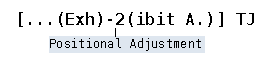
\includegraphics[width=2in]{tj.pdf}
    \caption{The TJ text showing operator, which specifies the glyphs to render and, by reference to a font object (not shown), their widths, along with any associated positional adjustments, given in text space units.}\label{fig:tj}
\end{figure}

The significant discovery of \emph{Story Beyond the Eye} was the existence and utilization of a novel redacted text information leak.
PDF documents can render text in numerous ways, including by use of a text showing operator, one of which (TJ) is depicted in Figure~\ref{fig:tj}. 
The TJ operator takes as arguments a string of text and a vector of \emph{positional adjustments} which displace the character with respect to a default position. 
This default position is usually a fixed offset from the previous character equivalent to the \emph{advance width} of the previous character defined elsewhere in the PDF document.

Glyph advance widths and glyph shifts create a security concern, and \emph{Story Beyond the Eye} found that most PDF redaction tools replace text selected for redaction with a single large shift of the same width as the redacted text showing operator, creating the two significant security risks:
\begin{itemize}
	\item The precise width of the redaction can be used to eliminate potential redacted texts, and is made more distinct than advance widths alone by glyph shifts.
	\item Any non-redacted glyph shifts conditioned on redacted glyphs can be used to eliminate potential redacted texts.
\end{itemize}
The work also addressed concerns related to nonexcising redactions. 
These redactions are cases where the text underneath the redaction can be selected and copied to the system clipboard from the PDF document.

Glyph shifts may then be classified as \emph{independent} or \emph{dependent}, where the former implies they are not determined by any particular character in the document, and the latter implies that they are---this is precisely dangerous if the character they are conditioned on is redacted.
This itself is not dangerous if the amount of information leaked on redacted text is small or the redaction tools themselves remove this information.
Thus, the methodology of the paper was split into extracting and evaluating glyph shifting schemes, e.g. from Microsoft Word's ``Save-as-PDF'' feature, and evaluating the information removed by redaction tools.

The latter corresponded to an evaluation of what types of information the redaction tools leaked, and after reverse engineering the schemes produced by 11 redaction tools, including Adobe Acrobat, the paper finds \emph{none} but those that rasterize the document entirely sufficiently mitigate these leaks.
Two of the tools were completely broken, and did not remove the text at all (created nonexcising redactions): the present author notified them of this problem and as a result of this both the tools have published patches.

\lstset{ %
language=C++,                % choose the language of the code
basicstyle=\ttfamily\footnotesize,       % the size of the fonts that are used for the code
numbers=left,                   % where to put the line-numbers
numberstyle=\footnotesize,      % the size of the fonts that are used for the line-numbers
stepnumber=1,                   % the step between two line-numbers. If it is 1 each line will be numbered
numbersep=5pt,                  % how far the line-numbers are from the code
backgroundcolor=\color{white},  % choose the background color. You must add \usepackage{color}
showspaces=false,               % show spaces adding particular underscores
showstringspaces=false,         % underline spaces within strings
showtabs=false,                 % show tabs within strings adding particular underscores
frame=single,           % adds a frame around the code
tabsize=2,          % sets default tabsize to 2 spaces
captionpos=b,           % sets the caption-position to bottom
breaklines=true,        % sets automatic line breaking
breakatwhitespace=false,    % sets if automatic breaks should only happen at whitespace
escapeinside={\%*}{*)}          % if you want to add a comment within your code
}

\begin{figure}
\begin{lstlisting}
for (int j = i + 1; j < vs->size(); j++) {
    t = ttfScaledWidths[j] / 1000;
    d = internalMSWordWidths[j] / internalMSWordFontSize;
    ttf += t;
    msWord += d;
    disp = ttf - msWord;
    if (((disp > 0.003) || (disp < -0.003)) && i != vs->size() - 1) {
      int adj = disp * 1000 + 0.5;
      vs->setShift(j, adj);
      ttf = msWord = 0;
    } else {
      vs->setShift(j, 0);
    }
}
\end{lstlisting}
\caption{Snippet of reverse engineered code representing how Microsoft Word leaks redacted character information into non-redacted characters in a PDF document.
    }
\label{fig:msword-snippet}
\end{figure}

The extraction and evaluation of the glyph shifting schemes involved precise tracing of PDF producer software and reverse engineering to extract an exact model of their positioning algorithms for text. 
Microsoft Word, in particular, provided glyph shift values that were \emph{highly} dependent on redacted glyphs, due to a floating-point error accumulation algorithm that compares the ``real'' PDF position of a glyph with a set of artificial positions determined by the full text of a given line.
A portion of this behavior, one of the error accumulators, is presented in Fig.~\ref{fig:msword-snippet}.
Note the internal widths used on line 3 of the figure are determined by a loop with no overflow reset and the redacted information held by the accumulator is not zero after a single shift is written: this detail is given in the publication's appendix.

The extraction of the prior algoithm and reverse engineering of PDF producer structures in a rich area and was not given sufficient space due to constraints on the original publication.
The proposed dissertation would provide both an explanation of how these algorithms were extracted as well as some of the challenges and solutions developed when addressing the problems of discovering and breaking redactions, and classifying glyph shifting schemes.

\subsubsection{Evaluation}

\paragraph{Synthetic Evaluation.}
The evaluation of the vulnerability these shifting schemes create for redacted text was based on the simulation of redactions on text from the New York Times annotated corpus~\cite{nytCorp} using various \emph{dictionaries}.
This represents how the amount of information leaked depends on prior information about the redacted text. 
For example, if we know the redacted text is one of 151,671 American surnames, then this redaction leaks at most $log_{2}(151, 671) \approx 17.2$ bits. 
Notably, these dictionaries included:



\renewcommand{\qedsymbol}{\rule{7pt}{7pt}}
\newcommand\maxray{Edact-Ray}

% The following macros give the pretty names of texts dictionaries and fonts.

\newcommand\wkpname{Wikipedia}
\newcommand\lawname{Legal}
\newcommand\nytname{News}

\newcommand\strname{Str}
\newcommand\acrnname{Acrn}
\newcommand\pronname{Pron}
\newcommand\wordname{Word}
\newcommand\fnname{FN}
\newcommand\lnname{LN}
\newcommand\filnname{FILN}
\newcommand\fixlnname{FI$\times$LN}
\newcommand\fnlnname{FNLN}
\newcommand\fnxlnname{FN$\times$LN}
\newcommand\ctryname{Ctry}
\newcommand\rgnname{Rgn}
\newcommand\natlname{Natl}

\newcommand\tfontname{Times}
\newcommand\afontname{Arial}
\newcommand\bfontname{Calibri}
\newcommand\rfontname{Courier}

\newcommand\nadjname{Unadjusted}
\newcommand\wxiiname{Word 2007}
\newcommand\wxxiname{Word 2021}

\newcommand\nadjshortname{Un}
\newcommand\wxiishortname{W07}
\newcommand\wxxishortname{W19}

\newcommand\uniname{Uniformly distributed}
\newcommand\empname{Text frequency distr.}

\newcommand\msWordPrefixMatch{XXX}

% wild section results
\newcommand\numWildCorpora{4}
\newcommand\numWildDNSALocSample{400}
\newcommand\numWildFOIALocSample{100}
\newcommand\numWildGovtLocSample{400}
\newcommand\numWildRECAPLocSample{100}
\newcommand\numWildLocSample{1,000}

\newcommand\dnsaNumDocs{678}
\newcommand\foiaNumDocs{1,580}
\newcommand\govtNumDocs{3,145}
\newcommand\recapNumDocs{\num{2.5e4}}
\newcommand\oigNumDocs{\num{1.9e4}}
% \newcommand\oigNumDocs{18,975}

% \newcommand\recapNumDocs{24,835}

\newcommand\dnsaPg{\num{1.2e4}}
% \newcommand\dnsaPg{12,498}
\newcommand\foiaPg{\num{4.9e5}}
% \newcommand\foiaPg{491,782}
\newcommand\oigPg{\num{5.2e5}}
% \newcommand\oigPg{515,870}
% \newcommand\govtPg{491,782}
\newcommand\recapPg{\num{3.4e5}}
% \newcommand\recapPg{336,973}

\newcommand\dnsaNonRastPg{8,628}
\newcommand\foiaNonRastPg{12,012}
\newcommand\govtNonRastPg{259,939}
\newcommand\recapNonRastPg{269,546}

% select corpus_name, count(distinct document_name) from redactions join pages
% on redactions.page = pages.hash group by corpus_name;
\newcommand\dnsaNumDocsWRedact{7}
\newcommand\foiaNumDocsWRedact{296}
\newcommand\govtNumDocsWRedact{230}
\newcommand\recapNumDocsWRedact{67}
\newcommand\totNumDocsWRedact{600}

\newcommand\totNumPagesWRedact{11,997}

% 112,149,773
\newcommand\numRECAPpages{$\approx10^{8}$}

\newcommand\avgShortlist{801}
\newcommand\avgNumNames{238}
\newcommand\avgStdDevRECAPName{1.3}

\newcommand\totalNonSynthNames{778}
\newcommand\numNonSynthRedactions{5,282}

\newcommand\numWildAttacked{769}

% select corpus_name, count(distinct redactions.id) from redactions 
% join pages on redactions.page = pages.hash group by corpus_name;
\newcommand\dnsaMetaRedact{235}
\newcommand\foiaMetaRedact{\num{4.5e4}}
\newcommand\oigMetaRedact{\num{1.3e4}}
% \newcommand\foiaMetaRedact{45,219}
% \newcommand\oigMetaRedact{13,214}
\newcommand\govtMetaRedact{51,651}
\newcommand\recapMetaRedact{1,221}
\newcommand\totMetaRedact{80,301}

\newcommand\unadjDNSA{7}
\newcommand\unadjFOIA{422}
\newcommand\unadjGOVT{2,589}
\newcommand\unadjRECAP{7}

\newcommand\ocrDNSA{0}
\newcommand\ocrFOIA{16,678}
\newcommand\ocrGOVT{3,939}
\newcommand\ocrRECAP{224}

\newcommand\mswDNSAExact{14}
\newcommand\mswFOIAExact{3}
\newcommand\mswGOVTExact{4,712}
\newcommand\mswRECAPExact{119}
\newcommand\mswDNSAExactFivePerc{7}
\newcommand\mswFOIAExactFivePerc{1}
\newcommand\mswGOVTExactFivePerc{1,428}
\newcommand\mswRECAPExactFivePerc{0}

\newcommand\mswDNSAExactTwelve{14}
\newcommand\mswDNSAExactTwenty{7}
\newcommand\mswFOIAExactTwelve{3}
\newcommand\mswFOIAExactTwenty{0}
\newcommand\mswGOVTExactTwelve{4,425}
\newcommand\mswGOVTExactTwenty{967}
\newcommand\mswRECAPExactTwelve{112}
\newcommand\mswRECAPExactTwenty{53}

\newcommand\mswDNSANear{3}
\newcommand\mswFOIANear{2}
\newcommand\mswGOVTNear{177}
\newcommand\mswRECAPNear{33}
\newcommand\mswDNSANearTwelve{0}
\newcommand\mswDNSANearTwenty{3}
\newcommand\mswFOIANearTwelve{1}
\newcommand\mswFOIANearTwenty{2}
\newcommand\mswGOVTNearTwelve{132}
\newcommand\mswGOVTNearTwenty{49}
\newcommand\mswRECAPNearTwelve{33}
\newcommand\mswRECAPNearTwenty{0}

\newcommand\unrecDNSA{214}
\newcommand\unrecDNSAUnkFont{32}
\newcommand\unrecDNSAKnwFont{182}
\newcommand\unrecFOIA{\num{1.3e4}}
% \newcommand\unrecFOIA{13,214}
\newcommand\unrecFOIAUnkFont{982}
\newcommand\unrecFOIAKnwFont{9,108}
\newcommand\unrecGOVT{40,270}
\newcommand\unrecGOVTUnkFont{6,468}
\newcommand\unrecGOVTKnwFont{33,802}
\newcommand\unrecRECAP{838}
\newcommand\unrecRECAPUnkFont{183}
\newcommand\unrecRECAPKnwFont{655}
\newcommand\unrecOIG{\num{1e4}}
% \newcommand\unrecOIG{10,517}

\newcommand\numWildTotalVuln{4,848}

\newcommand\nameDictSize{235,560}

\newcommand\numOIGUnmatched{39}

\newcommand\numRECAPPDFs{11,181,433}
\newcommand\numRECAPredactions{195,436}
\newcommand\numRECAPNameredactions{6,541}
\newcommand\numRECAPredactionDocs{710}

\newcommand\numRECAPnadj{327}
\newcommand\numRECAPnadjSample{100}
\newcommand\numRECAPocr{445}
\newcommand\numRECAPmsw{58}
\newcommand\numRECAPunk{5,691}
\newcommand\numRECAPNearMSW{20}

\newcommand\numRECAPtrivialRedaction{\num{1.9e5}}
%\newcommand\numRECAPtrivialRedaction{193,714}

\newcommand\nameDictSizeComb{7,066,800}

% ---
% Wild Results
% ---
\newcommand\dnsaExactName{XXX}
\newcommand\dnsaExactMrName{XXX}
\newcommand\dnsaExactMrsName{XXX}
\newcommand\dnsaExactFiLn{XXX}

\newcommand\foiaExactName{XXX}
\newcommand\foiaExactMrName{XXX}
\newcommand\foiaExactMrsName{XXX}
\newcommand\foiaExactFiLn{XXX}

\newcommand\govtExactName{XXX}
\newcommand\govtExactMrName{XXX}
\newcommand\govtExactMrsName{XXX}
\newcommand\govtExactFiLn{XXX}

\newcommand\recapExactName{XXX}
\newcommand\recapExactMrName{XXX}
\newcommand\recapExactMrsName{XXX}
\newcommand\recapExactFiLn{XXX}

\newcommand\hybridNadjAvgMatches{5,861}
\newcommand\hybridNadjMinMatches{10}

\newcommand\numFOIANamesAttacked{711}
\newcommand\numOIGNamesAttacked{58}

\newcommand\numFOIAUnmatched{382}
\newcommand\numFOIAUniq{3}
\newcommand\numOIGUniq{0}
\newcommand\numFOIAavg{2,435}
\newcommand\numFOIAmed{494}
\newcommand\numOIGavg{4,260}
\newcommand\numOIGmed{1,081}

\newcommand\foiaNameMaxRank{125,282}

\newcommand\avgMatchesWildTwo{561.09}
\newcommand\ratioNamesToMatches{420}
\newcommand\ratioWidthClassesToWidths{1095}

% ---
% Epstein Case Study
% ---

\newcommand\numEpsteinPagesRedacted{15}
\newcommand\numEpsteinDocuments{23}
\newcommand\numEpsteinRedactions{62}
\newcommand\numEpsteinVulnRedactions{4}


% The following macros give the dictionary sizes and uniform entropies. The names have
% the form
% 
%     \neltDDD  and  \hxDDD
% 
% where DDD is the dictionary, one of str, acrn, pron, word, fn, ln, filn, fnln, ctry, rgn, or natl


\input{defs0} % python tools/mkdefs0.py
% Overrides for prettier formatting. Always compare to actual numbers in defs0.tex.

\renewcommand\neltacrn{\num{1.2e7}}
\renewcommand\neltstr{\num{9e22}}
\renewcommand\neltfiln{\num{3.9e6}}
\renewcommand\neltfnln{\num{1.5e10}}
\renewcommand\neltrgn{\num{2.8e6}}
\newcommand\nelttsfnln{\num{1.8e6}}

% The following macros are for the word counts for each dictionary with respect to given
% text and the entropy of the dictionary distribution w.r.t. to a text. The names have
% the form
% 
%     \noccTTTDDD  and  \hxTTTDDD
% 
% where:
% 
% TTT is the text, one of wkp (Wikipedia), law (Legal), or nyt (News)
% DDD is the dictionary, one of str, acrn, pron, word, fn, ln, filn, fnln, ctry, rgn, or natl

\input{defs1} % python tools/mkdefs1.py

% The following macros are the results of the simulated redaction and guessing experiment. The
% names have the form
% 
%     \SSSMMMTTTDDDWWWFZ
% 
% where:
% 
% SSS is the statistic, one of hyu, hyw, hxyu, hxyw, puu, puw, pgu, pgw
% MMM is the static modifier, omitted or one of min, max, or avg
% TTT is the text, one of any (Any, unadj only), wkp (Wikipedia), law (Legal), or nyt (News)
% DDD is the dictionary, one of str, acrn, pron, word, fn, ln, filn, fnln, ctry, rgn, or natl
% WWW is the workflow, one of nadj (Unajusted), wxii (Word 2012), or wxxi (Word 2021)
% F is the font, one of t (Times), b (Calibri), a (Arial), or r (Courier)
% Z is the font size, one of ix (9 pt), x (10 pt), xi (11 pt), or xii (12 pt)
% 
% For example, \hyuavgnytfnnadjrxii is the average document residual entropy H(Y) for redactions
% on the News (NYT) corpus with first name dictionary, unadjusted text in 12 pt Courier.

\input{defs2} % python tools/mkdefs2.py
\input{defs3} % python tools/mkdefs3.py -t nyt blast


\begin{itemize}[nosep]
\item\textit{Str.} All strings of 3--16 characters in length starting with a uppercase or lowercase letter followed by lowercase letters.
\item\textit{Acrn.} All strings of 2--5 uppercase characters.
% \item\textit{Pron.} English third-person pronouns which are often redacted to avoid revealing a person's gender.
\item\textit{Word.} English words including some proper nouns.
\item\textit{Ctry.} Official and common names of countries.
\item\textit{Rgn.} Names of regions, a superset of \emph{Ctry}.
\item\textit{Natl.} Nationalities, demonyms, and adjectives of regions and nationalities, sourced from lists on Wikipedia.
\item\textit{FN.} American given (first) names.
\item\textit{LN.} American surnames (last names).
\item\textit{FI$\times$LN.} All combinations of a name initial followed by surname (\emph{LN}).
\item\textit{FN$\times$LN.} All combinations of a given name (\emph{FN}) followed by a surname (\emph{LN}).
\item\textit{FNLN and FILN.} \emph{FN$\times$LN} and \emph{FI$\times$LN} filtered to only include combinations of name and surname that appear in the voter registration databases of the three US states.
    North Carolina~\cite{ncVoterData}, Ohio~\cite{ohVoterData}, and Washington~\cite{waVoterData} were chosen based upon the availability of publicly accessible data.
\end{itemize}

\begin{table}
\centering
\caption{
    Dictionaries containing candidate texts used for evaluating deredaction. 
    Stop words are excluded from the statistics.
}\label{tab:dicts}
\small\begin{tabular}{lrr@{\hspace{3em}}*{1}{rr}}
\toprule
%& & 
%& \multicolumn{2}{c}{\emph{NYT}}
%\\
%\cmidrule(lr){4-5}
\emph{Dict.}
& \emph{Size}
& \emph{$H_{u}(X)$}
& \emph{NYT Occ.}
& \emph{$H_{e}(X)$}
\\
\midrule
\emph{Str} & \neltstr & \hxstr & \noccnytstr & \hxnytstr \\
\emph{Acrn} & \neltacrn & \hxacrn & \noccnytacrn & \hxnytacrn \\
% \emph{Pron} & \neltpron & \hxpron & \noccnytpron & \hxnytpron \\
\emph{Word} & \neltword & \hxword & \noccnytword & \hxnytword \\
\emph{Ctry} & \neltctry & \hxctry & \noccnytctry & \hxnytctry \\
\emph{Natl} & \neltnatl & \hxnatl & \noccnytnatl & \hxnytnatl \\
\emph{Rgn} & \neltrgn & \hxrgn & \noccnytrgn & \hxnytrgn \\
\emph{\fnname} & \neltfn & \hxfn & \noccnytfn & 10.3 \\
\emph{\lnname} & \neltln & \hxln & \noccnytln & 13.1 \\
  \emph{\filnname} & \num{1.6e6}      &   20.6  & 1,265,265 & 17.0 \\
\emph{\fixlnname} & \neltfiln & \hxfiln & \noccnytfiln & 17.0 \\
  \emph{\fnlnname} & \num{8.9e6}        &   23.1 & 3,650,063 & 19.6 \\  
\emph{\fnxlnname} & \neltfnln & \hxfnln & \noccnytfnln & 19.6 \\
\bottomrule
\end{tabular}

\end{table}

The amount of information leaked in the simulated redaction was measured both upon a uniform ($H_{u}(X)$) and empirical ($H_{e}(X)$) frequency distribution of each dictionary entry, i.e. one wherein the adversary knows which dictionary entries are more likely to occur and one wherein they treat each dictionary entry as equally possible.
It is therefore important to understand the size of these dictionaries and the number of bits of information they contain \emph{in total} with respect to both uniform and empirical distributions, so that the following synthetic evaluation results may be placed in context.
Scale measurements are given in Table~\ref{tab:dicts}.

\begin{table*}
\centering\small
\caption{Number of bits leaked (left) and probability of a correct guess (right) for different shifting schemes in simulated redactions of the NYT corpus set in 10pt font.
    Refer to Table~\ref{tab:dicts} for the total number of bits of information present in the candidate dictionary.
    ``Probability correct guess'' refers to the likelihood of randomly selecting the redacted word given the (typically small) set of matching candidate texts.
    }
\label{tab:nyt10}
\resizebox{0.89\width}{0.89\height}{
\newcommand\nytxunknown{\raisebox{1.25pt}{---}}
\begin{tabular}{l@{\hspace{0.785em}}l@{}r@{\hspace{3pt}}*{3}{@{\hspace{6pt}}*{3}{@{\hspace{1pt}}r@{\hspace{1pt}}}}@{\hspace{12pt}}*{3}{@{\hspace{6pt}}*{3}{@{\hspace{1pt}}r@{\hspace{2pt}}}}}
\toprule
& &
& \multicolumn{9}{c}{Leaked information (bits)}
& \multicolumn{9}{c}{Probability correct guess} \\
\cmidrule(lr){5-11}\cmidrule(lr){14-20}
\multicolumn{2}{l}{\emph{\textbf{Distr}}} & {Courier}\kern-8pt
& \multicolumn{3}{c}{{\tfontname}\hspace*{10pt}}
& \multicolumn{3}{c}{{\kern-6pt\afontname}}
& \multicolumn{3}{c}{{\kern-16pt\bfontname}}
& \multicolumn{3}{c}{{\tfontname}}
& \multicolumn{3}{c}{{\afontname}}
& \multicolumn{3}{c}{{\bfontname}}
\\
& \emph{Dict}
& Mo 
& {\nadjshortname} & {\wxiishortname} & {\wxxishortname}
& {\nadjshortname} & {\wxiishortname} & {\wxxishortname}
& {\nadjshortname} & {\wxiishortname} & {\wxxishortname}
& {\nadjshortname} & {\wxiishortname} & {\wxxishortname}
& {\nadjshortname} & {\wxiishortname} & {\wxxishortname}
& {\nadjshortname} & {\wxiishortname} & {\wxxishortname}
\\
\midrule
\multicolumn{6}{l}{\emph{\textbf{\uniname}}}
\\
& \emph{\strname}
& \hyunytstrnadjrx
& \hyunytstrnadjtx & \nytxunknown & \nytxunknown
& \hyunytstrnadjax & \nytxunknown & \nytxunknown
& \hyunytstrnadjbx & \nytxunknown & \nytxunknown
& \pgupctnytstrnadjtx & \nytxunknown & \nytxunknown
& \pgupctnytstrnadjax & \nytxunknown & \nytxunknown
& \pgupctnytstrnadjbx & \nytxunknown & \nytxunknown
\\
& \emph{\acrnname}
& \hyunytacrnnadjrx
& \hyunytacrnnadjtx & \hyuavgnytacrnwxiitx & \hyuavgnytacrnwxxitx
& \hyunytacrnnadjax & \hyuavgnytacrnwxiiax & \hyuavgnytacrnwxxiax
& \hyunytacrnnadjbx & \hyuavgnytacrnwxiibx & \hyuavgnytacrnwxxibx
& \pgupctnytacrnnadjtx & \pguavgpctnytacrnwxiitx & \pguavgpctnytacrnwxxitx
& \pgupctnytacrnnadjax & \pguavgpctnytacrnwxiiax & \pguavgpctnytacrnwxxiax
& \pgupctnytacrnnadjbx & \pguavgpctnytacrnwxiibx & \pguavgpctnytacrnwxxibx
\\
& \emph{\wordname}
& \hyunytwordnadjrx
& \hyunytwordnadjtx & \hyuavgnytwordwxiitx & \hyuavgnytwordwxxitx
& \hyunytwordnadjax & \hyuavgnytwordwxiiax & \hyuavgnytwordwxxiax
& \hyunytwordnadjbx & \hyuavgnytwordwxiibx & \hyuavgnytwordwxxibx
& \pgupctnytwordnadjtx & \pguavgpctnytwordwxiitx & \pguavgpctnytwordwxxitx
& \pgupctnytwordnadjax & \pguavgpctnytwordwxiiax & \pguavgpctnytwordwxxiax
& \pgupctnytwordnadjbx & \pguavgpctnytwordwxiibx & \pguavgpctnytwordwxxibx
\\
& \emph{\ctryname}
& \hyuavgnytctrynadjrx
& \hyuavgnytctrynadjtx & \hyuavgnytctrywxiitx & \hyuavgnytctrywxxitx
& \hyuavgnytctrynadjax & \hyuavgnytctrywxiiax & \hyuavgnytctrywxxiax
& \hyuavgnytctrynadjbx & \hyuavgnytctrywxiibx & \hyuavgnytctrywxxibx
& \pguavgpctnytctrynadjtx & \pguavgpctnytctrywxiitx & \pguavgpctnytctrywxxitx
& \pguavgpctnytctrynadjax & \pguavgpctnytctrywxiiax & \pguavgpctnytctrywxxiax
& \pguavgpctnytctrynadjbx & \pguavgpctnytctrywxiibx & \pguavgpctnytctrywxxibx
\\
& \emph{\rgnname}
& \hyuavgnytrgnnadjrx
& \hyuavgnytrgnnadjtx & \hyuavgnytrgnwxiitx & \hyuavgnytrgnwxxitx
& \hyuavgnytrgnnadjax & \hyuavgnytrgnwxiiax & \hyuavgnytrgnwxxiax
& \hyuavgnytrgnnadjbx & \hyuavgnytrgnwxiibx & \hyuavgnytrgnwxxibx
& \pguavgpctnytrgnnadjtx & \pguavgpctnytrgnwxiitx & \pguavgpctnytrgnwxxitx
& \pguavgpctnytrgnnadjax & \pguavgpctnytrgnwxiiax & \pguavgpctnytrgnwxxiax
& \pguavgpctnytrgnnadjbx & \pguavgpctnytrgnwxiibx & \pguavgpctnytrgnwxxibx
\\
& \emph{\natlname}
& \hyuavgnytnatlnadjrx
& \hyuavgnytnatlnadjtx & \hyuavgnytnatlwxiitx & \hyuavgnytnatlwxxitx
& \hyuavgnytnatlnadjax & \hyuavgnytnatlwxiiax & \hyuavgnytnatlwxxiax
& \hyuavgnytnatlnadjbx & \hyuavgnytnatlwxiibx & \hyuavgnytnatlwxxibx
& \pguavgpctnytnatlnadjtx & \pguavgpctnytnatlwxiitx & \pguavgpctnytnatlwxxitx
& \pguavgpctnytnatlnadjax & \pguavgpctnytnatlwxiiax & \pguavgpctnytnatlwxxiax
& \pguavgpctnytnatlnadjbx & \pguavgpctnytnatlwxiibx & \pguavgpctnytnatlwxxibx
\\
& \emph{\fnname}
& \hyunytfnnadjrx
& \hyunytfnnadjtx & \hyuavgnytfnwxiitx & \hyuavgnytfnwxxitx
& \hyunytfnnadjax & \hyuavgnytfnwxiiax & \hyuavgnytfnwxxiax
& \hyunytfnnadjbx & \hyuavgnytfnwxiibx & \hyuavgnytfnwxxibx
& \pgupctnytfnnadjtx & \pguavgpctnytfnwxiitx & \pguavgpctnytfnwxxitx
& \pgupctnytfnnadjax & \pguavgpctnytfnwxiiax & \pguavgpctnytfnwxxiax
& \pgupctnytfnnadjbx & \pguavgpctnytfnwxiibx & \pguavgpctnytfnwxxibx
\\
& \emph{\lnname}
& \hyunytlnnadjrx
& \hyunytlnnadjtx & \hyuavgnytlnwxiitx & \hyuavgnytlnwxxitx
& \hyunytlnnadjax & \hyuavgnytlnwxiiax & \hyuavgnytlnwxxiax
& \hyunytlnnadjbx & \hyuavgnytlnwxiibx & \hyuavgnytlnwxxibx
& \pgupctnytlnnadjtx & \pguavgpctnytlnwxiitx & \pguavgpctnytlnwxxitx
& \pgupctnytlnnadjax & \pguavgpctnytlnwxiiax & \pguavgpctnytlnwxxiax
& \pgupctnytlnnadjbx & \pguavgpctnytlnwxiibx & \pguavgpctnytlnwxxibx
\\
& \emph{\filnname}
 & 2.9 & 8.6 & 13.3 & 12.6 & 8.7 & 13.0 & 12.2 & 13.0 & 15.6 & 15.5 & <1\% & 4\% & 2\% & <1\% & 4\% & 2\% & 2\% & 11\% & 11\%
\\
& \emph{\fixlnname}
& \hyuavgnytfixlnnadjrx
& \hyuavgnytfixlnnadjtx & \hyuavgnytfixlnwxiitx & \hyuavgnytfixlnwxxitx
& \hyuavgnytfixlnnadjax & \hyuavgnytfixlnwxiiax & \hyuavgnytfixlnwxxiax
& \hyuavgnytfixlnnadjbx & \hyuavgnytfixlnwxiibx & \hyuavgnytfixlnwxxibx
& \pguavgpctnytfixlnnadjtx & \pguavgpctnytfixlnwxiitx & \pguavgpctnytfixlnwxxitx
& \pguavgpctnytfixlnnadjax & \pguavgpctnytfixlnwxiiax & \pguavgpctnytfixlnwxxiax
& \pguavgpctnytfixlnnadjbx & \pguavgpctnytfixlnwxiibx & \pguavgpctnytfixlnwxxibx
\\
& \emph{\fnlnname}
 & 3.2 & 9.4 & 14.5 & 14.1 & 10.0 & 14.9 & 14.0 & 13.5 & 16.7 & 16.5 & <1\% & 3\% & 2\% & <1\% & 4\% & 3\% & 3\% & 8\% & 7\%
\\
& \emph{\fnxlnname}
& \hyuavgnytfnxlnnadjrx
& \hyuavgnytfnxlnnadjtx & \hyuavgnytfnxlnwxiitx & \hyuavgnytfnxlnwxxitx
& \hyuavgnytfnxlnnadjax & \hyuavgnytfnxlnwxiiax & \hyuavgnytfnxlnwxxiax
& \hyuavgnytfnxlnnadjbx & \hyuavgnytfnxlnwxiibx & \hyuavgnytfnxlnwxxibx
& \pguavgpctnytfnxlnnadjtx & \pguavgpctnytfnxlnwxiitx & \pguavgpctnytfnxlnwxxitx
& \pguavgpctnytfnxlnnadjax & \pguavgpctnytfnxlnwxiiax & \pguavgpctnytfnxlnwxxiax
& \pguavgpctnytfnxlnnadjbx & \pguavgpctnytfnxlnwxiibx & \pguavgpctnytfnxlnwxxibx
\\
\multicolumn{6}{l}{\emph{\textbf{Text frequency distr.}}}
\\
& \emph{\strname}
& \hywnytstrnadjrx
& \hywnytstrnadjtx & \nytxunknown  & \nytxunknown
& \hywnytstrnadjax & \nytxunknown  & \nytxunknown
& \hywnytstrnadjbx & \nytxunknown  & \nytxunknown
& \pgwpctnytstrnadjtx & \nytxunknown & \nytxunknown
& \pgwpctnytstrnadjax & \nytxunknown & \nytxunknown
& \pgwpctnytstrnadjbx & \nytxunknown & \nytxunknown
\\
& \emph{\acrnname}
& \hywnytacrnnadjrx
& \hywnytacrnnadjtx & \hywavgnytacrnwxiitx & \hywavgnytacrnwxxitx
& \hywnytacrnnadjax & \hywavgnytacrnwxiiax & \hywavgnytacrnwxxiax
& \hywnytacrnnadjbx & \hywavgnytacrnwxiibx & \hywavgnytacrnwxxibx
& \pgwpctnytacrnnadjtx & \pgwavgpctnytacrnwxiitx & \pgwavgpctnytacrnwxxitx
& \pgwpctnytacrnnadjax & \pgwavgpctnytacrnwxiiax & \pgwavgpctnytacrnwxxiax
& \pgwpctnytacrnnadjbx & \pgwavgpctnytacrnwxiibx & \pgwavgpctnytacrnwxxibx
\\
& \emph{\wordname}
& \hywnytwordnadjrx
& \hywnytwordnadjtx & \hywavgnytwordwxiitx & \hywavgnytwordwxxitx
& \hywnytwordnadjax & \hywavgnytwordwxiiax & \hywavgnytwordwxxiax
& \hywnytwordnadjbx & \hywavgnytwordwxiibx & \hywavgnytwordwxxibx
& \pgwpctnytwordnadjtx & \pgwavgpctnytwordwxiitx & \pgwavgpctnytwordwxxitx
& \pgwpctnytwordnadjax & \pgwavgpctnytwordwxiiax & \pgwavgpctnytwordwxxiax
& \pgwpctnytwordnadjbx & \pgwavgpctnytwordwxiibx & \pgwavgpctnytwordwxxibx
\\
& \emph{\ctryname}
& \hywavgnytctrynadjrx
& \hywavgnytctrynadjtx & \hywavgnytctrywxiitx & \hywavgnytctrywxxitx
& \hywavgnytctrynadjax & \hywavgnytctrywxiiax & \hywavgnytctrywxxiax
& \hywavgnytctrynadjbx & \hywavgnytctrywxiibx & \hywavgnytctrywxxibx
& \pgwavgpctnytctrynadjtx & \pgwavgpctnytctrywxiitx & \pgwavgpctnytctrywxxitx
& \pgwavgpctnytctrynadjax & \pgwavgpctnytctrywxiiax & \pgwavgpctnytctrywxxiax
& \pgwavgpctnytctrynadjbx & \pgwavgpctnytctrywxiibx & \pgwavgpctnytctrywxxibx
\\
& \emph{\rgnname}
& \hywavgnytrgnnadjrx
& \hywavgnytrgnnadjtx & \hywavgnytrgnwxiitx & \hywavgnytrgnwxxitx
& \hywavgnytrgnnadjax & \hywavgnytrgnwxiiax & \hywavgnytrgnwxxiax
& \hywavgnytrgnnadjbx & \hywavgnytrgnwxiibx & \hywavgnytrgnwxxibx
& \pgwavgpctnytrgnnadjtx & \pgwavgpctnytrgnwxiitx & \pgwavgpctnytrgnwxxitx
& \pgwavgpctnytrgnnadjax & \pgwavgpctnytrgnwxiiax & \pgwavgpctnytrgnwxxiax
& \pgwavgpctnytrgnnadjbx & \pgwavgpctnytrgnwxiibx & \pgwavgpctnytrgnwxxibx
\\
& \emph{\natlname}
& \hywavgnytnatlnadjrx
& \hywavgnytnatlnadjtx & \hywavgnytnatlwxiitx & \hywavgnytnatlwxxitx
& \hywavgnytnatlnadjax & \hywavgnytnatlwxiiax & \hywavgnytnatlwxxiax
& \hywavgnytnatlnadjbx & \hywavgnytnatlwxiibx & \hywavgnytnatlwxxibx
& \pgwavgpctnytnatlnadjtx & \pgwavgpctnytnatlwxiitx & \pgwavgpctnytnatlwxxitx
& \pgwavgpctnytnatlnadjax & \pgwavgpctnytnatlwxiiax & \pgwavgpctnytnatlwxxiax
& \pgwavgpctnytnatlnadjbx & \pgwavgpctnytnatlwxiibx & \pgwavgpctnytnatlwxxibx
\\
& \emph{\fnname}
 & 2.5 & 7.1 & 9.3 & 9.0 & 7.2 & 8.8 & 8.6 & 9.7 & 10.0 & 9.9 & 45\% & 79\% & 74\% & 46\% & 71\% & 68\% & 87\% & 93\% & 92\%
\\
& \emph{\lnname}
 & 2.7 & 7.8 & 10.8 & 10.4 & 7.9 & 10.7 & 10.1 & 11.4 & 12.2 & 12.1 & 28\% & 59\% & 53\% & 28\% & 58\% & 51\% & 66\% & 81\% & 79\%
\\
& \emph{\filnname}
 & 2.7 & 8.4 & 12.4 & 11.9 & 8.5 & 12.2 & 11.5 & 12.6 & 14.4 & 14.3 & 8\% & 30\% & 22\% & 8\% & 25\% & 21\% & 34\% & 53\% & 52\%
\\
% & \emph{\fixlnname}
%  & 2.7 & 8.4 & 12.5 & 11.9 & 8.5 & 12.2 & 11.5 & 12.6 & 14.4 & 14.3 & 8\% & 30\% & 22\% & 8\% & 25\% & 21\% & 34\% & 53\% & 52\%
% \\
& \emph{\fnlnname}
 & 3.1 & 9.2 & 13.8 & 13.6 & 9.8 & 14.3 & 13.5 & 13.2 & 15.9 & 15.8 & 4\% & 20\% & 19\% & 6\% & 24\% & 19\% & 16\% & 38\% & 37\%
\\
% & \emph{\fnxlnname}
%  & 3.1 & 9.2 & 13.8 & 13.6 & 9.8 & 14.3 & 13.5 & 13.2 & 15.9 & 15.8 & 4\% & 20\% & 19\% & 6\% & 24\% & 19\% & 16\% & 38\% & 37\%
% \\
\bottomrule
\end{tabular}
}

\end{table*}

The results of this synthetic evaluation are given in Table~\ref{tab:nyt10}.
Note that four different fonts and three glyph shifting schemes were evaluated: Courier presents a strawman result for a purely monospaced font with no shifts.
The \emph{Un} column presents the efficacy of deredaction provided an attack utilizing the width of the PDF text alone, if no adjustments occur.
This is a specific case of an \emph{independent} shifting scheme.
The \emph{W07} and \emph{W19} columns present the Microsoft Word shifting schemes in the 2007 and 2019 desktop versions of Microsoft Word.
These, in turn, depict changes in the algorithm over time and highlight the historical significance of the attack, as it has been possible in documents over the range of at least a decade.

\paragraph{Real Evaluation.}
The present author also evaluated the extent of information leaks in real documents, using the following corpora, which were attained using a combination of webscraping and redaction location algorithms.
The latter were custom-made, and included separate algorithms for excising and nonexcising redactions.
Both were constructed to identify single-color boxes in-between and on top of text, respectively.

\begin{enumerate}
    \item \emph{FOIA.} Documents obtained via the US Freedom of Information Act (FOIA) on governmentattic.org~\cite{govattic}. 
This corpus provides us with independently selected documents with some public interest.
    \item \emph{OIG.} Office of the Inspector General (OIG) reports hosted by oversight.gov~\cite{oigReports}. 
The OIG is a US Government oversight branch tasked with preventing unlawful operation of other government branches.
This corpus allowed us to measure the impact deredaction may have on documents from a high-profile and large organization.
    \item \emph{DNSA.} Digital National Security Archive (DNSA) documents produced after 2010~\cite{dnsaSite}. 
The DNSA is a set of historical US government documents curated by scholars. 
That is, we found redaction information leaks affect significant historical documents.
    \item \emph{RECAP.} CourtListener's RECAP court document archive.
RECAP mirrors PACER, the US Federal Courts' docketing system~\cite{pacerSite}, and contains over 10 million documents.
We use RECAP to measure the impact of nonexcising redactions (discussed below).
    \item \emph{rRECAP} the subset of RECAP documents returned for the search string ``redacted''.
We chose to include rRECAP because running the excising redaction location algorithm mentioned in on the entire RECAP corpus would be both computationally and financially prohibitive.
\end{enumerate}

Only the RECAP corpus contained nonexcising redactions and our results for this corpus were reported with respect to nonexcising redactions.
Our results for all other corpora were reported with respect to excising redactions.

In this evaluation it was necessary to correctly infer the specific glyph shifting scheme of each document and whether that document was vulnerable, thus a framework for classifying a redaction was developed.
This framework included the additional constraint that the redaction could be reasonably classified as a name, in order to reduce the false positives rate created by attempting deredaction on entries outside the evaluated dictionary, FN$\times$LN.
A real-world redaction was evaluated if either:
\begin{enumerate}[nosep]
    \item The redacted text is present in the PDF (vulnerable to copy-paste attack); or
    \item The redacted text is not present, but the document retains glyph shifting scheme information where:
        \begin{itemize}[nosep]
            \item The scheme matches a Word ``Save as PDF'' shifting scheme,
            \item The redaction appears to be a name, e.g. ``Jane'', and
            \item The redaction is the first from left to right on the line of text.
        \end{itemize}
\end{enumerate}

\begin{table}
  \centering
    \caption{Top: Glyph shifting schemes identified in redacted corpora pages. Bottom: Deredaction results for names tagged.}
\label{tab:wildres}
\small%\begin{tabular}{l@{\hspace{-3pt}}r@{\hspace{6pt}}r@{\hspace{3pt}}r@{\hspace{3pt}}r|r}
\begin{tabular}{lrr@{\hspace{3pt}}r@{\hspace{3pt}}r|r}
  \toprule
    Metric             & FOIA              & OIG              & DNSA                & rRECAP               & RECAP                     \\
  \midrule
Documents          & 3,145             & \oigNumDocs           & \dnsaNumDocs        & \recapNumDocs        & $\approx10^{7}$           \\
  Pages              & \foiaPg           & \oigPg          & \dnsaPg             & \recapPg             & \numRECAPpages            \\
  % Non-raster Pages &                   &                  &                     &                      & RECAP                     \\
  Redacted PDFs      & 236               & 1255             & \dnsaNumDocsWRedact & \recapNumDocsWRedact & \numRECAPredactionDocs    \\
  %Redacted Pages    & XXX               & XXX              & XXX                 & XXX                  & XXX                       \\
  Redactions         & \foiaMetaRedact & \oigMetaRedact & \dnsaMetaRedact     & \recapMetaRedact     & \numRECAPNameredactions   \\
  \ Unadjusted     & 2,844             & 314              & \unadjDNSA          & \unadjRECAP          & \numRECAPnadj             \\
  \ Adobe OCR      & 3,406             & 1,814            & \ocrDNSA            & \ocrRECAP            & \numRECAPocr              \\
  \ Near Word   & 175               & 114              & \mswDNSANear        & \mswRECAPNear        & \numRECAPNearMSW          \\
  \ Unrec.   & \unrecFOIA &  \unrecOIG         & \unrecDNSA          & \unrecRECAP          & \numRECAPunk              \\
  \ Exact Word     & 4,694             & 455              & \mswDNSAExact       & \mswRECAPExact       & \numRECAPmsw              \\
  Vulnerable       & 711               & 58               & 9                   & 0                    & \numRECAPmsw              \\
  \midrule
    No Matches          & \numFOIAUnmatched & \numOIGUnmatched & 1                  & --                   & N/A                        \\
  Uniq. Matches      & \numFOIAUniq      & \numOIGUniq      & 5                  & --                   & N/A                        \\
  Avg. Matches        & \numFOIAavg       & \numOIGavg       & 393                  & --                   & N/A                        \\
  Med. Matches        & \numFOIAmed       & \numOIGmed       & 1                  & --                   & N/A                        \\
  \bottomrule
\end{tabular}

%   \begin{tabular}{l@{\hskip -3cm}lrrrr}
%     \toprule
%     \multicolumn{2}{l}{}                               & \emph{DNSA}                & \emph{FOIA}                      & \emph{Govt.}          & \emph{RECAP}                                                   \\
%     \midrule
%     \multicolumn{2}{l}{Documents}                      & \dnsaNumDocs               & xxx  & \govtNumDocs          & \recapNumDocs                                                  \\
%     \multicolumn{2}{l}{Pages}                          & \dnsaPg                    & xxx  & \govtPg               & \recapPg                                                       \\
%     \multicolumn{2}{l}{Non-raster pages}               & \dnsaNonRastPg             & xxx  & \govtNonRastPg        & \recapNonRastPg                                                \\
%     \multicolumn{2}{l}{Redacted docs}                  & \dnsaNumDocsWRedact        & xxx  & \govtNumDocsWRedact   & \recapNumDocsWRedact                                           \\
%     \midrule
%     \multicolumn{2}{l}{Redacted text objs.}            & \dnsaMetaRedact            & xxx  & \govtMetaRedact       & \recapMetaRedact                                               \\
%                                                        & Unadjusted                 & xxx  & \unadjFOIA            & \unadjGOVT                            & \unadjRECAP            \\
%                                                        & Adobe OCR                  & xxx  & \ocrFOIA              & \ocrGOVT                              & \ocrRECAP              \\
%                                                        & Exact MS Word (>100 chars) & xxx  & \mswFOIAExact         & \mswGOVTExact                         & \mswRECAPExact         \\
%                                                        & Exact MS Word (<5\% error) & xxx  & \mswFOIAExactFivePerc & \mswGOVTExactFivePerc                 & \mswRECAPExactFivePerc \\
% %    \multicolumn{2}{l}{\ \ Exact 2012}                & \mswDNSAExactTwelve        & xxx  & \mswGOVTExactTwelve   & \mswRECAPExactTwelve                                           \\
% %    \multicolumn{2}{l}{\ \ Exact 2021}                & \mswDNSAExactTwenty        & xxx  & \mswGOVTExactTwenty   & \mswRECAPExactTwenty                                           \\
%                                                        & Near MS Word               & xxx  & \mswFOIANear          & \mswGOVTNear                          & \mswRECAPNear          \\
% %    \multicolumn{2}{l}{\ \ Near 2012}                 & \mswDNSANearTwelve         & xxx  & \mswGOVTNearTwelve    & \mswRECAPNearTwelve                                            \\
% %    \multicolumn{2}{l}{\ \ Near 2021}                 & \mswDNSANearTwenty         & xxx  & \mswGOVTNearTwenty    & \mswRECAPNearTwenty                                            \\
%                                                        & Unrecognized adj.          & xxx  & \unrecFOIA            & \unrecGOVT                            & \unrecRECAP            \\
% %    \multicolumn{2}{l}{\ \ Unknown font}              & \unrecDNSAUnkFont          & xxx  & \unrecGOVTUnkFont     & \unrecRECAPUnkFont                                             \\
% %    \multicolumn{2}{l}{\ \ Known font}                & \unrecDNSAKnwFont          & xxx  & \unrecGOVTKnwFont     & \unrecRECAPKnwFont                                             \\
%     \midrule
%     uncor names\_all                                   &                            & 0/2 (0.0\%), 0/0, 1/2 (50.0\%)   & xxx & 42/626 (6.7\%), 19/232 (8.2\%), 0/0   & 0/0, 0/0, 0/0          \\
% uncor mr\_surnames                                     &                            & 1/1 (100.0\%), 0/0, 1/2 (50.0\%) & xxx & 19/296 (6.4\%), 11/122 (9.0\%), 0/0   & 0/0, 0/0, 0/0          \\
% uncor mrs\_surnames                                    &                            & 0/0, 0/0, 0/0                    & xxx & 16/210 (7.6\%), 2/79 (2.5\%), 0/0     & 0/0, 0/0, 0/0          \\
% uncor names\_all\_straight\_pos                        &                            & 1/1 (100.0\%), 0/0, 0/0          & xxx & 7/57 (12.3\%), 2/20 (10.0\%), 0/0     & 0/0, 0/0, 0/0          \\
% uncor names\_all\_curly\_pos                           &                            & 0/0, 0/0, 0/0                    & xxx & 16/218 (7.3\%), 3/83 (3.6\%), 0/0     & 0/0, 0/0, 0/0          \\
% uncor ameng                                            &                            & 0/2 (0.0\%), 0/0, 1/2 (50.0\%)   & xxx & 47/604 (7.8\%), 19/227 (8.4\%), 0/0   & 0/0, 0/0, 0/0          \\
% uncor countries                                        &                            & 0/0, 0/0, 1/1 (100.0\%)          & xxx & 81/128 (63.3\%), 33/50 (66.0\%), 0/0  & 0/0, 0/0, 0/0          \\
% uncor demonyms                                         &                            & 0/0, 0/0, 2/2 (100.0\%)          & xxx & 69/98 (70.4\%), 25/30 (83.3\%), 0/0   & 0/0, 0/0, 0/0          \\
% cor names\_all                                         &                            & 0/2 (0.0\%), 0/0, 1/2 (50.0\%)   & xxx & 46/460 (10.0\%), 19/152 (12.5\%), 0/0 & 0/0, 0/0, 0/0          \\
% cor mr\_surnames                                       &                            & 1/1 (100.0\%), 0/0, 1/2 (50.0\%) & xxx & 19/249 (7.6\%), 11/90 (12.2\%), 0/0   & 0/0, 0/0, 0/0          \\
% cor mrs\_surnames                                      &                            & 0/0, 0/0, 0/0                    & xxx & 16/190 (8.4\%), 2/70 (2.9\%), 0/0     & 0/0, 0/0, 0/0          \\
% cor names\_all\_straight\_pos                          &                            & 1/1 (100.0\%), 0/0, 0/0          & xxx & 7/57 (12.3\%), 2/20 (10.0\%), 0/0     & 0/0, 0/0, 0/0          \\
% cor names\_all\_curly\_pos                             &                            & 0/0, 0/0, 0/0                    & xxx & 18/168 (10.7\%), 5/52 (9.6\%), 0/0    & 0/0, 0/0, 0/0          \\
% cor names\_all,mr\_surnames                            &                            & 0/2 (0.0\%), 0/0, 0/2 (0.0\%)    & xxx & 48/554 (8.7\%), 22/188 (11.7\%), 0/0  & 0/0, 0/0, 0/0          \\
% cor names\_all,mrs\_surnames                           &                            & 0/2 (0.0\%), 0/0, 1/2 (50.0\%)   & xxx & 40/535 (7.5\%), 15/186 (8.1\%), 0/0   & 0/0, 0/0, 0/0          \\
% cor names\_all,names\_all\_straight\_pos               &                            & 0/2 (0.0\%), 0/0, 1/2 (50.0\%)   & xxx & 49/488 (10.0\%), 22/162 (13.6\%), 0/0 & 0/0, 0/0, 0/0          \\
% cor names\_all,mr\_surnames,names\_all\_straight\_pos  &                            & 0/2 (0.0\%), 0/0, 0/2 (0.0\%)    & xxx & 51/579 (8.8\%), 24/197 (12.2\%), 0/0  & 0/0, 0/0, 0/0          \\
% cor names\_all,mrs\_surnames,names\_all\_straight\_pos &                            & 0/2 (0.0\%), 0/0, 1/2 (50.0\%)   & xxx & 43/557 (7.7\%), 17/194 (8.8\%), 0/0   & 0/0, 0/0, 0/0          \\
% cor names\_all,names\_all\_curly\_pos                  &                            & 0/2 (0.0\%), 0/0, 1/2 (50.0\%)   & xxx & 51/524 (9.7\%), 19/176 (10.8\%), 0/0  & 0/0, 0/0, 0/0          \\
% cor names\_all,mr\_surnames,names\_all\_curly\_pos     &                            & 0/2 (0.0\%), 0/0, 0/2 (0.0\%)    & xxx & 49/603 (8.1\%), 22/210 (10.5\%), 0/0  & 0/0, 0/0, 0/0          \\
% cor names\_all,mrs\_surnames,names\_all\_curly\_pos    &                            & 0/2 (0.0\%), 0/0, 1/2 (50.0\%)   & xxx & 44/587 (7.5\%), 16/206 (7.8\%), 0/0   & 0/0, 0/0, 0/0          \\
% cor ameng                                              &                            & 0/2 (0.0\%), 0/0, 1/2 (50.0\%)   & xxx & 52/450 (11.6\%), 18/154 (11.7\%), 0/0 & 0/0, 0/0, 0/0          \\
% cor countries                                          &                            & 0/0, 0/0, 1/1 (100.0\%)          & xxx & 81/83 (97.6\%), 30/31 (96.8\%), 0/0   & 0/0, 0/0, 0/0          \\
% cor demonyms                                           &                            & 0/0, 0/0, 2/2 (100.0\%)          & xxx & 76/79 (96.2\%), 25/25 (100.0\%), 0/0  & 0/0, 0/0, 0/0          \\
% \midrule
%     Correlated FN/LNs                                  &                            & \dnsaExactName                   & xxx & \govtExactName                        & \recapExactName        \\
%     FNLN Cases                                         &                            & \dnsaExactName                   & xxx & \govtExactName                        & \recapExactName        \\
%     Matched FNLNs                                      &                            & \dnsaExactName                   & xxx & \govtExactName                        & \recapExactName        \\
%     \midrule
%     Total Exact                                        &                            & \dnsaExactName                   & xxx & \govtExactName                        & \recapExactName        \\
%     True Positive Exact                                &                            & \dnsaExactName                   & xxx & \govtExactName                        & \recapExactName        \\
%     False Positive Exact                               &                            & \dnsaExactName                   & xxx & \govtExactName                        & \recapExactName        \\
%     \bottomrule
%   \end{tabular}

\end{table}

The resulting evaluation broke hundreds of redactions in real world documents. 
The results of this are reported in Table~\ref{tab:wildres}.
It is important to note the definition of \emph{broke}: the FN$\times$LN dictionary contained $1.5 \times 10^{10}$ entries, so a reduction to a few hundred or thousands possibilities is significant.
We confirmed with affected parties that often the feasible dictionary is much smaller, and the results for $FNLN$ in Table~\ref{tab:nyt10} emphasize the attack is dangerous.
Many additional verifications of these findings were performed but are omitted from this proposal due to space constraints.

\subsubsection{Discussion}

Due to the complex technical matter of deredaction and methodological novelties in the evaluation of deredaction attacks, the original publication did not include a description of technical facets of modeling glyph shifting schemes that are essential to correct deredaction.
The extraction of glyph shiftng schemes from Microsoft Work, Adobe Acrobat, and other systems was non-trivial and the present author was forced to perform this modeling and reverse engineering largely manually.

One important feature of these algorithms was their dependence on floating point error: they could not be lifted to continuous equations without resulting in an incorrect representation.
This is deeply related to the assumptions made in the InteGreat work, which ignores floating point error when lifting continuous control equations from binary firmware for the purposes of verification.
Clearly there are domains wherein this floating point error is and is not \emph{useful}, and the proposed dissertation will address this problem in a greater depth by contrasting the two works, something the works, independently considered, could not discuss.

The other key success (and limitation) of \emph{Story Beyond the Eye} was the paper's treatment of the unknown: deredaction may never be considered as determining the correct redacted text, but only as ruling out possibilities with the assumption that the observed evidence is complete, correct, and correctly understood.
The paper also highlights important notions core to the use of leaked or remaining information after information destruction (redaction) occurs, most notably the notion of a \emph{prior}, provided by a dictionary.
These ideas are, to the present author's knowledge, hardly discussed in the context of lifting and binary program analysis, and both the Jetset and InteGreat works would have benefitted from a richer comprehension of this facet of information loss.
The proposed dissertation will more closely consider the role that prior information may play in the domains of firmware rehosting and continuous equation lifting.


\subsection{InteGreat}

InteGreat reinterprets bitvector-domain symbolic execution of program slices into the theory of uninterpreted functions to perform modular, nestable function summarization and lifting.
The tool provides researchers with a novel design language for automatically abstracting complex programs into mathematical equations.
In the submitted publication, InteGreat's lifting was used to determine the sensor inputs necessary to precisely destabilize the reactor pressure of a chemical plant, discover novel problems in the domain of firmware rehosting, and discover a flaw in the implemented version of a published quad-copter stabilization algorithm.

\subsubsection{Motivating Example}

To introduce InteGreat's core contributions, compare the typical operation of symbolic execution on a function in a closed-source binary firmware to InteGreat's approach.

\begin{figure}
  \centering
	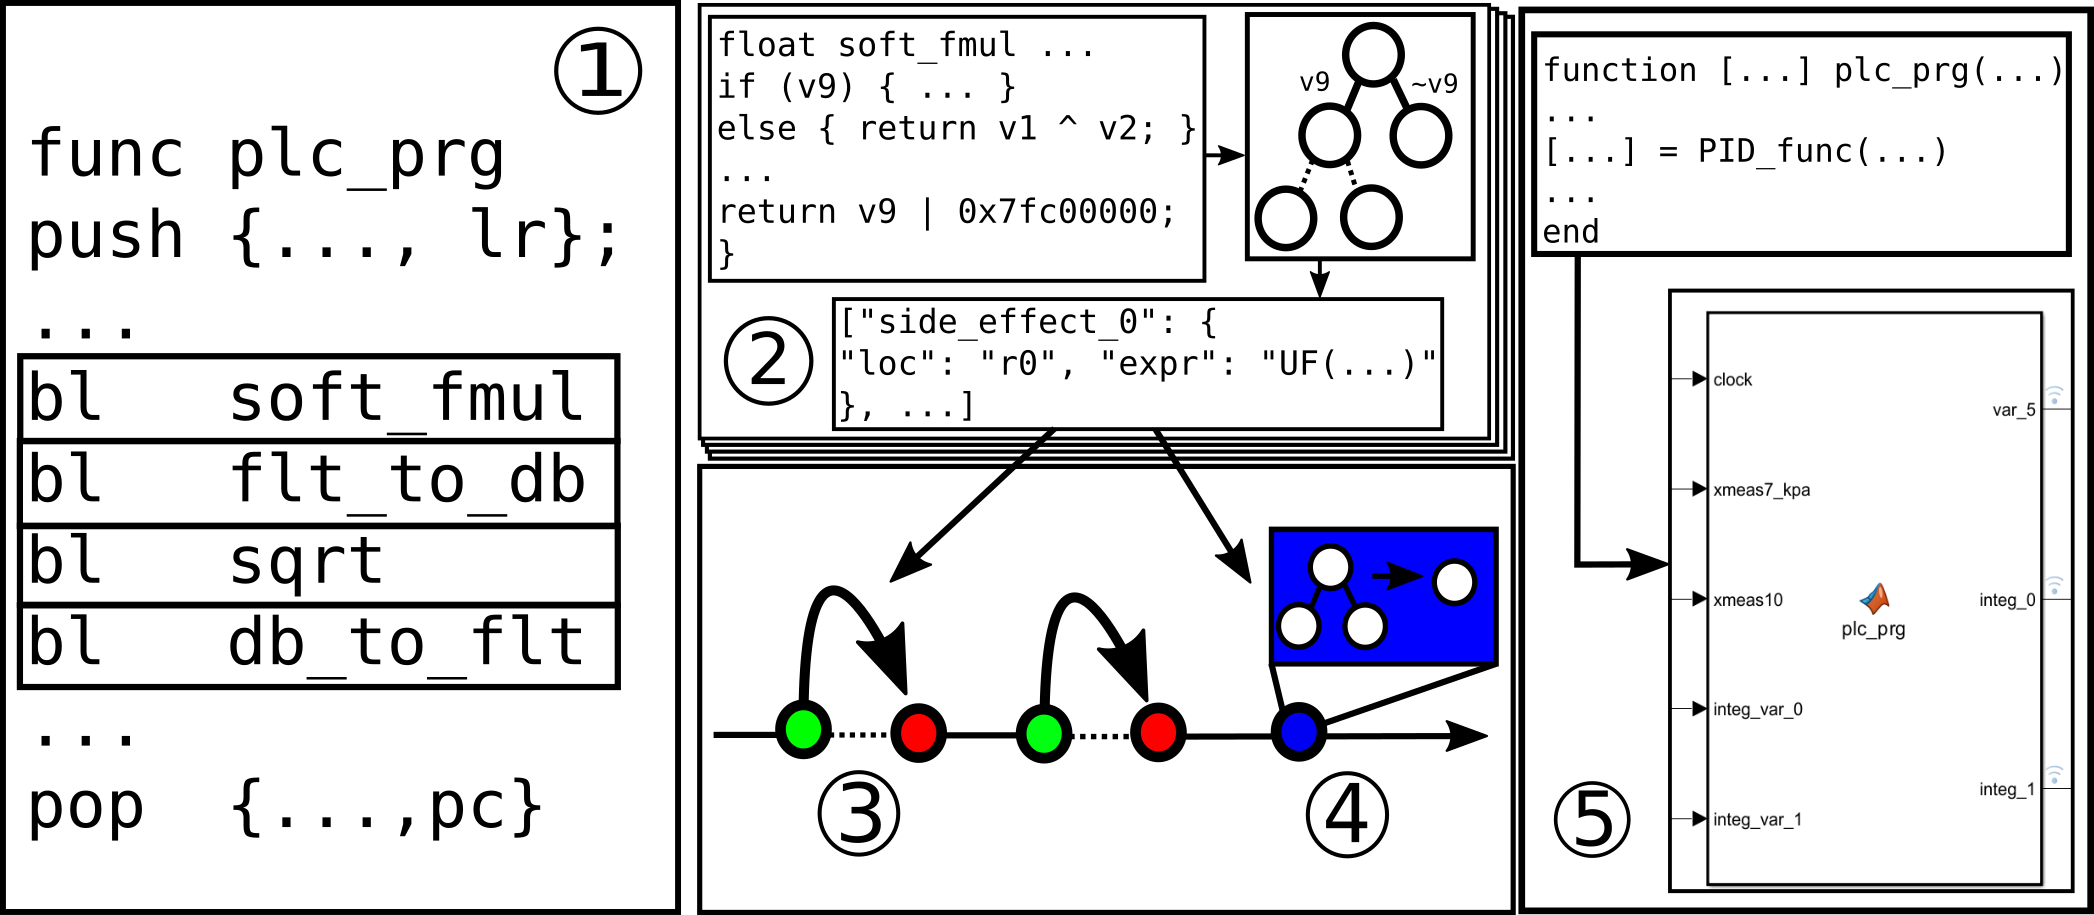
\includegraphics[width=0.7\textwidth]{integreat-example.png}
	\caption{Depiction of an example execution of InteGreat on a small program. Red/Green nodes describe abstracting a program slice. Blue stands for program slice pattern triggering higher level abstractions that stitches slices according to combination rules}
	\label{fig:integreat-example}
\end{figure}

\paragraph{Traditional Symbolic Execution.}
Traditional symbolic execution of the function presented in (1) of Fig.~\ref{fig:integreat-example} will begin by loading a symbolic state $S$ at the entry point to the function.
Between each inner call, a number of additional instructions could exist but are not depicted.
Upon reaching a child function, symbolic execution will enter this function and begin to execute it.
The symbolic executor will then proceed to accumulate all the branches, constraints, and operations in the child function.
A software floating point multiply we studied, for example, had 153 lines of pseudo-C, 116 of decompiled assembly, and 15 branches.
The symbolic executor will then exit the child function and begin executing the succeeding instruction with some $n$ possible symbolic constraint sets.
This process will continue until the end of the program is reached.
Finally, in most cases, the symbol executor will output a statement over the theory of bitvectors rather than a more abstract domain, due to the complexity of determining relevant or desired abstraction boundaries in the general case.

Complexity arises due to the lack of a general solution to the halting problem and the necessity of supporting various microarchitectural operational semantics.
A loop without an explicit guard condition within a child function may entirely sabotage symbolic execution due to \emph{state explosion}.
For example, a while-true loop may have a break condition which could fire on any of $1\dots\infty$ iterations (this is common during reads from hardware devices).
Moreover, angr~\cite{angr-1} and to our knowledge most other closed-source binary symbolic executors do not (publicly) support memory accesses to a symbolic address, as these may potentially reference the entire address space, leading to a combinatorial explosion of the possible resulting execution states. 
This issue was solved by Coppa et al.~\cite{coppa2017rethinking}, however, it was never integrated into angr~\cite{angr-2}.

\paragraph{InteGreat's Approach.} Unlike a traditional symbolic executor, InteGreat adopts a more constrained goal of lifting to continuous equations that can be loaded into a mathematical verifier or program like Matlab.
To achieve this, InteGreat provides users with a mechanism for associating program slices to symbols, and handles all the semantic ``stitching'' this entails automatically.
We assume the control flow of a given slice is completely contained within another and there may be no partial overlaps (an independence system).
A simple example of this would be the address range of a function compiled inline into the body of another function, or a call instruction itself. 
The largest slice is the program itself, and slices consist of entry and exit addresses.

First, in (1), we begin a post-order tree traversal of the program slices, descending to ``leaf'' program slices that have no inner slices. 
For simplicity, in Fig.~\ref{fig:integreat-example} we define the slices as each inner function, called to by each \emph{bl} assembly instruction.
These slices are provided to InteGreat via a JSON specification file.

Then, in (2), we generate an \emph{abstraction specification} for each given slice.
We use traditional symbolic execution to identify all the possible side-effect locations (registers, memory) of the slice for each execution path, which includes function input locations.
Note that here we have assumed the desired semantics for the slice's computation are decidable given some \emph{search strategy}.

To avoid state explosion when lifting undecidable algorithms, we leave this strategy user-configurable but provide a few sensible defaults, e.g. taking the state that generates the most complex set of constraints or the largest number of writes to memory.
However, state explosion remains a hard problem for abstract interpretation and InteGreat helps to make progress on this problem by providing a more general interface for abstracting program slices.
To cope with the problem of combinatorial pointer value explosion discussed above, we implement a version of the 2017 Coppa et al. work, representing each read or write to memory with both the value and the symbolic expression used to determine the address, discussed below.

Next, in (3), we begin the process of \emph{abstraction resolution}.
Assuming all $n$th layer slices are correctly lifted and the symbolic execution state is loaded at the beginning of each slice in the $n+1$th layer.
Symbolic execution proceeds as normal until it hits the entry point of an $n$th layer program slice $\gamma$.
In the simplest case, the symbolic execution jumps to the exit point of this slice and parameterized uninterpreted function(s) $f$ are written to the output location(s) of $\gamma$.
To parameterize $f$, the constraints and execution context at the input locations of $\gamma$ (locations are identified in (2)) are supplied as parameters to $f$.
$f$ does not have to be an uninterpreted function, but could be any (recovered) model of the child slice's semantics.
(3) continues until a higher level abstraction is triggered or the function ends (e.g. return).

(4) represents how each exit point of a program slice triggers a check for patterns specified as higher level abstractions.
Upon each pattern match, a corresponding rewrite rule is applied to the abstract symbol tree (AST) containing the symbolic constraints for the current program execution path.
This allows us, for instance, to automatically abstract out the marshalling of bitvectors to and from register pairs necessary to represent 64-bit floating point values on 32-bit architectures.

In (5) we post-process the resultant AST, linking output expressions to inputs and resolving abstractions into a model in a high-level language. 
In this paper, we target Matlab code as it provides an easy, reproducible evaluation.
At this stage, program slices are ordered by symbolic execution timestamps, and we disambiguate different pointer values passed into the same program slice using the strict equality discussed above.
Finally, we also parse side-effects into stateful variables, i.e. self-loops from output to input.
We also remove duplicate computations (AST subtrees) across multiple outputs by translating the AST into a sequence of assignments.

\subsubsection{Techniques}

InteGreat reformulates classical function summarization (introduced in Sec.~\ref{sec:func-summarization}) as \emph{nested function summarization}.
A nested function summarization is of the form $\Gamma_1, \Gamma_2 \ \ldots \ \Gamma_n$, where every $\Gamma$ is a non-empty finite set of dynamic logic formulas. 
Nested function summarizations can be reused and \emph{chained} inside of higher-level summarizations.
The decision procedure for such resolutions follows from $\Gamma$.

In order to define a nested function summarization $\Gamma$ in domain $\mathcal{D}$, we split $\Gamma$ into two sets, $\Gamma_{M}$ and $\Gamma_{S}$, representing the \emph{storage} and \emph{semantics} (expressions) of a program slice, respectively.
Given $m \in M$, $\Gamma_{M} \vdash m_{\mathcal{M}} \rightarrow m'_{\mathcal{D}}$, binding the symbols for registers and memory to the abstract domain, and $\Gamma_{S} \vdash S^{\Gamma}_{\mathcal{M}} \rightarrow S'_{\mathcal{D}}$, where $S^{\Gamma}_{\mathcal{M}} \subseteq S_{\mathcal{M}}$, a partial mapping of the semantics of the concrete domain to equivalent semantics in the abstract domain.
Partial specification allows users to avoid, for example, reproducing the microarchitecture. A given usecase may only require semantics indicated by \texttt{call} instructions.
$\Gamma$ may then be specified for new domains $\mathcal{D}, \mathcal{D}', \ldots$ by substituting $\mathcal{M}$ for the higher layer of abstraction.

We define program slices as abstraction boundaries that occur naturally in the firmware or by user definition.
Each abstraction or summarization is a decision to associate a \emph{sign} (a fresh symbolic variable) with a specific set of computations.
The set of substituted instructions, i.e. the range of summarization, must be \emph{complete}: all the program semantics which should be substituted for $f$ must be substituted ($S^{f}_{\mathcal{M}} \subseteq S^{\Gamma}_{\mathcal{M}}$).
This, for example, could require resolving the callsites indicated by dynamically assigned pointer values, something that is hard to do generally, as these values could be I/O dependent: InteGreat addresses this problem by requiring the abstraction of program slices invoking the virtual call (otherwise it will throw a fault).
Although in general this problem is also solvable using other means, e.g. symbolically executing more of the program or by using static analysis.

As a computation $S$ can have loops, we must ensure or assume that the nested function summarization $\Gamma$ is \emph{closed}, i.e. the set of operations $S^{\Gamma}_{\mathcal{M}}$ is finite.
The basic solution in cases where $S$ halts for all inputs is universal quantification or the computation of a \emph{fixed point}.
For example, let $T = \{t_{1}, t_{2}, \ldots, t_{n}\}$ be the complete set of possible traces over computations $C =c_{1}, c_{2}, \ldots, c_{n}$ in the program slice.
Then the summarization $\Gamma$ is closed if $\Gamma \vdash \bigwedge_{t \in T} \Gamma_{S} \vdash t_{\mathcal{M}} \rightarrow t'_{\mathcal{D}}$.
To allow analysis of $S^{C}_{\mathcal{M}} \notin HALT$, we use a \emph{search strategy}.
In prior work the search strategy is a bound $v$ for unrolling all loops in $S$ (Sec.~\ref{sec:func-summarization}).

\textbf{Nested Abstraction Resolution.} 
  \label{prob:abstraction-resolution}
Once the particular side-effects of a program slice are \emph{bound}, the side-effect values upon exiting the slice may be substituted with arbitrary logical operations over the program's state, similar to a standard SimProcedure in angr.
Unlike angr, InteGreat automates the nesting of procedures based upon a formula, so that more complex abstractions may be built from simpler ones.
Representing a function $f$, we construct $\Gamma \vdash S^{f}_{\mathcal{M}} \rightarrow S^{f}_{\mathcal{D}}$, but the concrete domains $\mathcal{M}$ includes abstractions previously defined by $\Gamma$ and $\mathcal{D}$ is not itself ``hard-coded'' but defined by the logical formulae used to substitute the program slices (either automatically lifted uninterpreted functions or user-specified alternative formulae for the slices' semantics).
However, any concrete implementation must restrict $\mathcal{D}$ to some finite set of supported syntaxes, e.g. QF\_UF.
InteGreat supports the same theories as Z3.


\lstdefinelanguage{json}{
    basicstyle=\footnotesize\ttfamily,
    showstringspaces=false,
    breaklines=true,
    float=tp,
    numbers=none,
    floatplacement=tbp
}

\lstset{language=json,basicstyle=\ttfamily\scriptsize}
\begin{figure}
\begin{lstlisting}
"pid": {"addrs": [<auto-populated, e.g. 0xCAFE:0xCBFE], "conf": "./pid.json"}
"derivative": {"addrs": [<auto-populated>], "conf": "./derivative.json"}
"integral": {"addrs": [<auto-populated>], "conf": "./integral.json"}
\end{lstlisting}
\vspace{5pt}
\hrule\vspace{5pt}
\begin{lstlisting}
"in":   {"i0":{"type": "float", "location": "reg", "ptr": "r0"},
         "i1":{"type": "float", "location": "reg", "ptr": "r1"}},
"out":  {"o0":{"type": "float", "location": "reg", "ptr": "r0"},
"expr": "(declare-fun F((_FloatingPoint 8 24)) Bool) ...
	(declare-funinput()(_BitVec32))(...)...
		assert(let((a!1(...(_ to_fp 8 24) i1)..."
\end{lstlisting}
% "absts"     : ['mul.json', 'integral.json', 'atan.json'],
% "out"   : {"o0": {"type": "float", "location": "stack", "ptr": "S+8"},
%            "o1": {"type": "float", "location": "mem", "ptr": "M[0x2004]+8"}},
% \begin{lstlisting}
% "slices":     [{"addr":"0xcafe:0xcaff"}],
% \end{lstlisting}
\vspace{5pt}
\hrule\vspace{5pt}
\begin{lstlisting}
"slice_expr": "f2d, muldf, trunc",
"abst_in":    {"f2d":["i0"], "muldf":["i2", "i3"]},
"abst_out":   {"trunc":["o0"]},
\end{lstlisting}
	\caption{\textbf{Top}: Example of a top-level configuration file, with symbolic execution specifications connected to a list of inference rules. \textbf{Middle}: InteGreat automatically exports this function summarization of a derivative function as a Z3 function expression with bindings to the input locations. \textbf{Bottom}: Example higher-order inference rules with references to nested program slices, used to rewrite multiplication function with type conversion to plain multiplication.} 
\label{fig:json-example}
\end{figure}

\textbf{Input.}
\label{sec:input-output}
The input to InteGreat is a firmware $F$ and a set of program slices.
Slices can take the form of a range of addresses (potentially of zero length), a type of instruction, or an expression over the names of other slices.
To avoid repeating the same abstraction in multiple places, we break this up into a set of objects, where the ``entrypoint'' object refers to the highest level of abstraction, and descendants refer to inner slices.

The top of Figure~\ref{fig:json-example} provides the list of program slices.
\emph{These slices and the JSON file hierarchy can be automatically generated from static analysis of $F$, and InteGreat provides a set of scripts covering basic use cases, e.g. abstract every child function of a given function.}
Thus, in the figure we list the addresses for the slices as ``auto-populated''.
However, we leave the decision to use auto-population scripts to the user, to avoid assumptions about $F$'s structure and the desired abstractions.

As InteGreat executes, each JSON file is populated with the inference rules $(\mathcal{I}$, $\mathcal{A})$ for lifting the program slice.
A simplified version of these outputs are given in the middle of Figure~\ref{fig:json-example}.
Importantly, it contains three parts: the input variables supplied to the inference, the side-effect locations (outputs), and the expression for the slice reinterpreted as an uninterpreted function.
Optionally, because this expression is a logical formula over the program state, the user can \emph{modify} this file after the fact and specify alternative or additional formulae for abstracting the program slice.

Finally, once inference rules $(\mathcal{I}, \mathcal{A})$ are generated for sub-slices, we allow these abstractions to be composed at runtime.
An example of this is shown in the bottom of Figure~\ref{fig:json-example}, which is used to tell InteGreat to compose the given abstractions into a single multiply over the reals, rather than an operation over bitvectors with type conversions.



% For an end-summarization $\Gamma$, the inputs are in the form of $\Gamma_{M} \vdash m_{\mathcal{M}} \rightarrow m'_{\mathcal{D}}$, binding the symbols for registers and memory to the abstract domain.
% $\Gamma$ outputs are always in the form of $\Gamma_{S} \vdash S^{\Gamma}_{\mathcal{M}} \rightarrow S'_{\mathcal{D}}$, binding abstract domain to registers and memory.
%The free variables of $S$ are dynamically interpreted in $\mathcal{I}$, depending on the underlying axioms of symbolic exectution state $x$.

\label{fig:json-abst-example}
\textbf{Output.}
The output of InteGreat is a vastly simplified Z3 AST composed mainly of uninterpreted functions.
The structure of the program slices is decided such that translating the recovered control equations to MATLAB or \LaTeX\ is trivial, and InteGreat includes scripts for this purpose.

% \subsection{Overview}
% 
% \label{sec:overview}
% InteGreat operates on program slices, which are a range of instructions in the firmware. 
%  On each program slice, InteGreat performs transformation from the underlying program slice into a higher-level representation of the underlying computation.
% 
% At the lowest level, InteGreat performs symbolic execution on the program slice and extracts basic semantics of the original program. 
%  During Symbolic Exectution using angr~\cite{angr}, InteGreat leverages program transformations to address challenges in Symbolic Execution.
%  One of the common challenges of applying Symbolic Execution in program transformation is handling branches and loops, since Symbolic Execution only explores a single path at a time, generating expression sets with information from a single execution path. 
%  To extract models from firmware, we need to perserve the branching information, effectively merging the execution traces of all paths into a single expression.
%  InteGreat has two main approaches: (i) Use director strategies to guide the symbolic execution engine to explore interesting paths, and (ii) Use transformation mechanism to provide a higher-level expression for a program slice that contains branching.  
%  For example, if-then-else blocks can be transformed into a constant value, effectively removing the branch condition.
% 
%  InteGreat also allows users to define transformations upon other transformations to compose higher-level representations using results of other representations.
%  One example is a program slice calculating $\sqrt{a^2+b^2+c^2}$ using the abstractions "square" and "sqrt" can be replaced with a single function calculating euclidean distance.
%  Function composition can also be replaced with a single function call.
%  This is accomplished through data-flow analysis on dynamic Symbolic Exectution tracking connections between program slice transformations.
% 
%  When working with control functions, users mark integral and derivative functions and InteGreat replaces them with an expression with automatically inferred inputs.
%  InteGreat includes tool scripts to automate describing transformations.
%  The following example illustrates this process from Section ~\ref{sec:plc}.

 %Specifically InteGreat provides Ghidra scripts to facilitate defining transformations for program slices associated with interesting functions.
 %The user can use any underlying tool to supply a firmware, architectural information, entry point of the function, function calling conventions,  which memory regions need to be concrete, SE path search strategy.
 %The user may open up the firmware in Ghidra and manually identify a control loop core function.

% First the user obtains firmware containing the calculation of interest.
% The user then uses Ghidra or other reverse enginer to identify the function of interest.
% In the TE PLC, pid\_fixcycle is located at xxx, this step requires manual effort, but it is out of scope for this paper.
%



%when SE chooses a single execution path when reaching branches or loops, and accumulates constraints and expressions describing that path.

%One of the challenges faced by prior work is that SE only accumulates constraints and expressions on one single program path, and branching information that manifests in the constraint set are lost in the expressions.  
 



%\label{sec:overview}
%This section explains the main workflow of InteGreat.
%A high-level overview of the workflow is shown in Figure ~\ref{fig:integreat-strategy}.
%Detailed description of algorithms and implementation are in ~\ref{sec:algorithms}.
%
%In \emph{Static Analysis} stage, configuration files are generated by the user.
% The user locates an entry point in the firmware, and specifies the set of abstractions and their inference rules to be applied, as shown in Figure ~\ref{fig:json-example}.
% \textbf{Note that we are not solving the decision procedure of where to place abstractions, instead, we solve the problem of providing a tool to facilitate that decision procedure}.
%
%In \emph{Abstract Interpretation} stage, InteGreat runs an augmented Symbolic Execution Engine based on ANGR \cite{angr} developed on ANGR's event hook infrastructure and implements symbolic memory.
% Each time an augmented event hook with matching interpretation rules in the user configurations is triggered to pause symbolic execution.
% The \emph{Sequent Inference Algorithm} explained in ~\ref{sec:algorithms} is performed, and then symbolic execution continues with its program state updated.
% InteGreat does not directly expose its abstract interpretation results to ANGR, instead, InteGreat supplies abstraction symbolic variables at the abstraction output locations, and records inference results.
% Inference results are stored as symbolic expression trees with high-level abstractions as leaf ASTs.
%
%
%% \emph{Sequent Inference} takes in the current symbolic execution state and the current sequent configuration, dynamically evaluates the set of user supplied operations.
%% The inference result is not seen by the symbolic execution engine, however, the symbolic state needs to be updated to reflect the side effects of the abstraction.
%% For example, some abstractions perform modifications on the program state, as register values may be changed after a function is called. 
%% In such situations, we supply fresh place-holder symbolic values describing the abstraction to the symbolic execution state where the abstraction performs program state modifications, and record timestamps.
%% For higher level \emph{Sequent Inferences} that modify previous Sequent Inference results and do not directly modify the program state, we promptly perform modifications on the stored inference results instead of the program state.
%%Thus, symbolic execution continues, operating on abstraction symbolic variables until the termination condition is reached, deriving expression sets operating on abstractions.
%
%The \emph{Abstraction Resolution} stage of InteGreat takes in the expression sets derived from the first stage.
% We name the resulting high-level expression set our goal sequent $\Gamma_{goal}$.
% InteGreat performs the \emph{Abstraction Resolution Algorithm} as explained in ~\ref{sec:algorithms} on the goal sequent $\Gamma_{goal}$.
% \emph{Abstraction Resolution} applies concretion on $\Gamma_{goal}$ using sequent inference results on the subsequents. 
% The resulting expression set $\mathcal{E}$ now consist of Z3 ~\cite{Z3} expressions with each variable bound to the concrete program state $\mathcal{M}$, and are associated with timestamps listed in SSA form.
% $\mathcal{E}$ is exported in a JSON specification format that can be directly used as input to InteGreat.
% It is now straight-forward to lift these Z3 expressions to control equations presented in MATLAB or other verifiable form, handled by the \emph{Translators}.
%
%InteGreat's implementation of abstract interpretation addresses several challenges in symbolic execution.
%Path explosion is a common problem in symbolic execution when over-approximations of loops and other branching conditions introduce too much path complexity.  
%InteGreat leverages function summarization to replace complex over-approximations with a single abstraction, reducing the number of symbolic execution paths generated.
%The \emph{Search Strategy Algorithm} explained in ~\ref{sec:algorithms} also offers search strategies to chooses the most appropriate symbolic execution path to explore.
%Therefore, InteGreat merges states in symbolic execution, and performs symbolic execution on the merged state.

% All functions are implemented in Python 3.9.

% 2. \emph{Sequent Inference Algorithm} - This algorithm is used to perform sequent inference on the symbolic execution state.
% 3. \emph{Abstraction Resolution Algorithm} - This algorithm is used to perform abstraction resolution on the sequent inference results.
% 4. \emph{Director Algorithm} - This algorithm is used to perform symbolic execution on the merged state.

% Hooks & symbolic memory
\renewcommand{\algorithmicrequire}{\textbf{Input:}}
\renewcommand{\algorithmicensure}{\textbf{Output:}}

\begin{algorithm}
    \caption{Abstraction Lifting}
    \begin{algorithmic}[1]
        \footnotesize
	\Require S, $\mathcal{E}$
        \Ensure $\mathcal{E}'$
        \State \ldots \algorithmiccomment{Symbolically execute slice $S$, recovering $m_{in},m_{out}$}
        \For{\textbf{each} \texttt{i} \textbf{in} $m_{in}$} \algorithmiccomment{Bind concrete input to abstract expressions}
        \State $m \leftarrow \mathcal{M}(i)$
        \State $\mathcal{B}_{in}(m) \leftarrow MEM\_READ(m)$ \algorithmiccomment{query InteGreat's symbolic memory model}
        \EndFor
        \For{\textbf{each} \texttt{o} \textbf{in} $m_{out}$} \algorithmiccomment{Bind abstract expressions to concrete output}
        \State $m \leftarrow \mathcal{M}(o)$
        \State $e \leftarrow \mathcal{E}(o)$
        \State $\mathcal{B}_{out}(m) \leftarrow e$
        \EndFor
        \For{\textbf{each} b \textbf{in} $\mathcal{B}_{out}$}
        \State $v \leftarrow NEW\_ABST()$
        \State $MEM\_WRITE(b, v)$ \algorithmiccomment{Write abstraction to angr's symbolic memory}
        \State $\mathcal{T}(v) \leftarrow TIMESTAMP$
        \EndFor

    \State $\mathcal{E}' \leftarrow BIND(\mathcal{E}, \mathcal{B}_{in}, \mathcal{B}_{out})$\algorithmiccomment{Bind inference result expressions to outputs}

        \State $\mathcal{E}' \leftarrow SORT(\mathcal{E}', \mathcal{T})$\algorithmiccomment{Sort by timestamp}
        \For{\textbf{each} o \textbf{in} $\mathcal{B}_{out}$}
	    \State $\mathcal{E}' \leftarrow APPLY(\Gamma, o, \mathcal{E}')$\algorithmiccomment{Recursively substitute abstractions}
        \EndFor
    \end{algorithmic}
    \label{alg:abst-binding}
\end{algorithm}

\textbf{Abstraction Lifting Algorithm.}
\label{sec:algorithms}
Algorithm~\ref{alg:abst-binding} handles lifting from symbolic variables in $\mathcal{M}$ to $\mathcal{D}$.
 Input to this algorithm is the set of expressions $\mathcal{E}$, the current recovered abstract semantics of the program in $\mathcal{D}$ and inference rules $\mathcal{I}$ (by default, for lifting to a single uninterpreted function), and the desired program slice to abstract, $S$.
 The output is a new state $\mathcal{E}'$ with bindings $\mathcal{B}$ applied to InteGreat's implementation of Symbolic Memory.

InteGreat first retrieves a set of registers and memory locations $m_{\{in,out\}} \in \mathcal{M}$ describing the microarchitectural input and output locations of a program slice.
These are provided via a symbolic executor with modifications to support the use of symbolic values as memory addresses.
For locations with existing symbolic expressions, InteGreat's symbolic memory dynamically fetches the most recent written expression, or else InteGreat writes and returns a fresh symbolic variable in that location.

InteGreat then dereferences the input locations to the correct symbolic expressions representing their values in InteGreat's symbolic memory model (the inputs may be sets of previously lifted abstractions), and \emph{binds} them into the inputs of the desired abstraction $\mathcal{E}$.
InteGreat replaces the existing lower-level, concrete expressions returned by symbolic execution for the slice's outputs with the higher higher-level abstraction via the binding $\mathcal{B}_{out}$.

The last step establishes the lifting results as fresh abstractions to the symbolic memory state.
The abstraction is maintained by linking $\mathcal{B}$ into a new lifted program state $\mathcal{E}'$.
All future symbolic execution and calls to Alg.~\ref{alg:abst-binding}, will operate on the abstractions provided by $\mathcal{B}_{out}$ rather than the original concrete symbolic expression for each $m_{out}$.

Consider, for example, a floating point multiply over registers $r_{0}$ and $r_{1}$, with output in $r_{0}$.
A set of operations are recovered for symbolic inputs $i_{0}$ and $i_{1}$, yielding the symbolic output $o_{0} = i_{0} * i_{1}$.
%TODO: This example needs to come much sooner. Like in the introduction.  Its where I start to see the pieces come together.
%TODO: You could start with a simple example of recovering a simple floating point operation from assembly, to recovering equations.  (Maybe start with multiplication, as it should be simple and nearly obvious how to transform from assembly to real domain.  Then move to an example where it only takes an additional step two, but it is not immediately apparent how to do it Perhaps integration)
A fresh symbolic variable $abst\_mul\_o0$ would be created and written to the symbolic memory model at concrete register location $r_{0}$, and the output of this algorithm would be $\mathcal{E} \cup r_{0} = new\_sym \mapsto abst\_mul\_o0(i_{0},i_{1})$ rather than $\mathcal{E} \cup r_{0} = i_{0} * i_{1}$.


%  Consider an example $\mathcal{I}$, specified in the middle part of Figure ~\ref{fig:json-example}.
%  $m_{\mathcal{M}}$ references register locations r0 and r1, and dynamically infers the symbolic expressions binded with r0 and r1 through querying InteGreat's symbolic memory.
%  r0 and r1 may not be bound to any symbolic expression, and InteGreat returns a fresh symbolic variable.
%  r0 and r1 may also already contain a symbolic expression from a previous symbolic execution path, and InteGreat returns the existing symbolic expression.
%  As a result, microarchitectural locations r0 and r1 in $\mathcal{M}$ are now binded to symbolic expressions in $\mathcal{D}$.
%  
% The user provides (i) lambdas in the form of $\Gamma_{M} \vdash m_{\mathcal{M}} \rightarrow m'_{\mathcal{D}}$ or $\Gamma_{S} \vdash S_{\mathcal{D}} \rightarrow S'_{\mathcal{D}}$  for inputs, (ii) Statements $S$ in SSA form operating on symbolic placeholders of inputs for assignments.

% The input expressions when in nested $\Gamma_{S}$ form, allows $S$ to operate on the inputs and outputs of $\Gamma$s as a higher level abstraction.
% and (iii) lambdas $\Gamma_{S} \vdash S^{\Gamma}_{\mathcal{M}} \rightarrow S'_{\mathcal{D}}$, for outputs.
% The input lambda expressions $m_{\mathcal{M}} \vdash H(x,\ell)$ are derived from the dynamic symbolic state.
% These derived $\Gamma_{M}$ are then substituted into the symbolic placeholders of the user supplied $S$, yielding $S'$ which is the actual function summarization of this abstraction.
% The output of this algorithm is the finalized expression set $S'$.

% The first step either takes in a set of program operations $S$ and uninterpreted function expressions $UF$.
% Both $S$ and $UF$ map from the inputs of the abstraction to the outputs of the abstraction. 
% However, we must transform $S$ and $UF$ into a set of output expressions $\mathcal{E}$ with all free variables corresponding to the input inference rules.
% We ensure $S$,$UF$ are formatted in single static assignment (SSA) form, so we can recursively \emph{flatten} the SSA assignment map until all output expressions $\mathcal{E}$ correspond to inference output rules.
%  \emph{SSA Flattening} refers to removing intermediate assignment steps via substitution with their corresponding expressions in the SSA assignment map.
%  Both $S$ and $UF$ are now a mapping of context-insensitive symbolic expressions to abstraction outputs, and all free variables in the expressions corresponding to abstraction inputs.
%   
% The next step is binding the context-insensitive symbolic expressions summarizing functions to the symbolic execution context. 
%  If the inference input rules $(\mathcal{I}, \mathcal{A})$ contain concrete program state specifications, the \emph{Abstraction Binding} is applied.
%  This procedure lifts concrete inputs into the abstract domain, and records the set of bindings $\mathcal{B}$ in InteGreat's symbolic memory model.
%  If the inputs are already abstract, these lifting rules are applied using the names of upon sub-abstractions that are nested in this abstraction.
% \toolname\ guarantees, correctly, that all abstractions eventually resolve into operations on the program state, by recording abstractions into InteGreat's symbolic memory model through the mappings provided by the recovered side-effects of sub-abstractions.
%  Now all inference inputs are mapped to symbolic expressions in the abstract domain $\mathcal{D}$.
%  To bind inference outputs to the symbolic expressions in $\mathcal{E}$, we perform $\alpha$-renaming on the symbolic expressions in $\mathcal{E}$ to inherit the context of dynamically inferred inputs.
%  Thus, the context-insensitive function summaries inherit context-related information from the inference inputs.
 
 
%The output statements $\Gamma_{S} \vdash S^{\Gamma}_{\mathcal{M}} \rightarrow S'_{\mathcal{D}}$ are obtained from the flattening the SSA statements $S'$ in $\Gamma$.
%The temporary assignments are recursively substituted in the output statements, yielding the final output statements.
%The output locations to the $s$ are described as $\Gamma_{M} \vdash m_{\mathcal{D}} \rightarrow m'_{\mathcal{M}}$.
%A fresh symbolic variable denoting each output is created and written into the output locations.
%The fresh symbolic variable is associated with the output expression in $S'$, stored in a local data structure $\mathcal{L}$, which is the output of this algorithm.

The last step of Algorithm~\ref{alg:abst-binding}, lines 17 through 20, is a backward chaining inference algorithm applied on the final expression sets in the derived AST.
The lifted program state $\mathcal{E}'$ and a set of expressions for lifting other abstractions described as lambda functions $\Gamma_{S} \vdash S^{\Gamma}_{\mathcal{M}} \rightarrow S'_{\mathcal{D}}$ in user configuration files (see ``slice\_expr'' in Fig.~\ref{fig:json-example}) are applied to resolve output locations into higher-order abstractions.
In this process, InteGreat leverages timestamps to ensure that the abstractions are resolved in the correct order.

\label{sec:symb-mem-expl}
\textbf{Symbolic Memory.}
An important part of the InteGreat workflow is describing input and output locations for each abstraction to obtain symbolic expression trees.
 In most firmware programs, inputs and outputs are context-sensitive to its program state, for example, the dynamic execution stack, or a dereferenced pointer to a memory location.
 Thus it is necessary for InteGreat to allow symbolic expressions as memory addresses.

InteGreat accomplishes this by implementing a symbolic memory model, extending Trt{\'\i}k et al.'s model~\cite{symbolic-memory}, under-constrained memory ~\cite{Under-Constrained}, and incorporating the core ideas of Coppa et al.~\cite{coppa2017rethinking}.
Leveraging the angr event hook infrastructure, InteGreat intercepts all program state modifications, and replaces them with InteGreat's symbolic memory model. 
During each pointer dereference, the symbolic memory model is queried with the intercepted dynamic state of Symbolic Execution.

Memory Aliasing implemented by proving the equivalence of expressions for pointer addresses.
When resolving memory, we use the timestamps of each memory operation and a strict equivalence check on the pointer expression to determine when a memory location is modified.
So, for example if $p_{1} = 50$ and $p_{2} = 50$, and we are checking $read(p_{1}) = write(p_{2})$, then we will return that they are NOT the same memory location. 
That is, we do not assume runtime knowledge. 
We assume that if such knowledge is needed, a zero-size program slice (an entry point address equivalent to the exit address) will be defined that will identify this runtime equivalence, and other tools exist for this~\cite{hind2001pointer}.

\subsubsection{Evaluation}

We evaluated InteGreat by recovering equations for continuous orientation estimation from an open-source, MCU-based quad-copter autopilot controller~\cite{drone}. 
The firmware we studied implemented Madgwick's Gradient Descent Orientation Filter \cite{madgwick}.
Madgwick provided a C-code implementation of this algorithm in the cited publication.

We also extracted continuous equation models from a PLC controlling a pressure-controlling valve in the Tenessee Eastman Challenge~\cite{Tennessee-Eastman}, a benchmark for modeling and analyzing the dynamics of industrial control systems.
The firmware for this PLC was provided by the ICSREF~\cite{ICSREF} paper, an security paper which staged a code upload attack on a physical PLC connected to a Matlab environmental model.
Additional details of this attack's physical setup are given in~\cite{keliris2016machine}.

\begin{figure*}
    \centering
    \begin{subfigure}[b]{0.327\textwidth}
        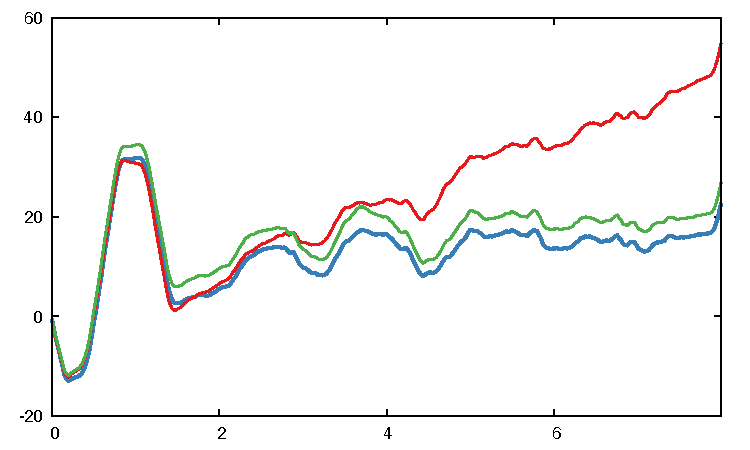
\includegraphics[width=\textwidth]{madg_data/pitch.pdf}
	    \caption{Pitch}
    \label{fig:pitch}
    \end{subfigure}
    \hfill
    \begin{subfigure}[b]{0.327\textwidth}
        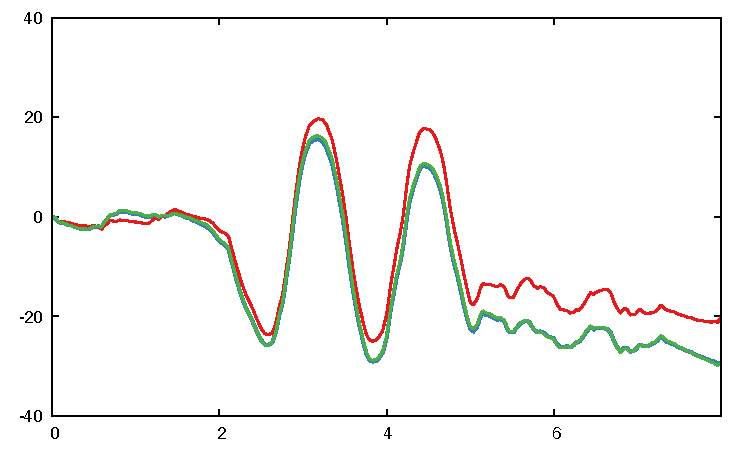
\includegraphics[width=\textwidth]{madg_data/yaw.pdf}
        \caption{Yaw}
        \label{fig:yaw}
    \end{subfigure}
    \hfill
    \begin{subfigure}[b]{0.327\textwidth}
        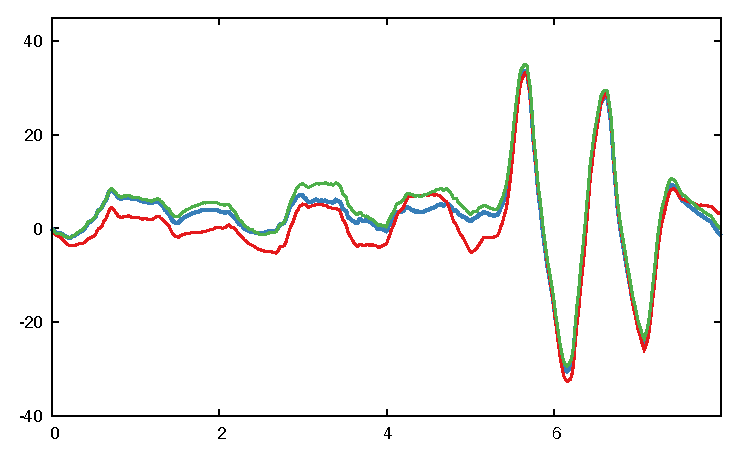
\includegraphics[width=\textwidth]{madg_data/roll.pdf}
        \caption{Roll}
        \label{fig:roll}
    \end{subfigure}
    \hfill
    \caption{Experimental Results: Orientation Estimation of a device oscillating in pitch, yaw, then roll. \textbf{Green} is lifted by InteGreat from \emph{real world} firmware that contains a bug. \textbf{Blue} contains \emph{two} lines: the InteGreat lifted firmware recompiled to correct the gradient calculation, and \emph{a correct} Matlab implementation of Madgwick's algorithm. \textbf{Red}, however, is a compiled firmware using the \emph{faulty} C code included in Madgwick's published report. This version has accumulative error with respect to the earth's magnetic field.}
    \label{fig:madg}
\end{figure*}

\textbf{Quadcopter}
We ran four experiments using different versions of Madgwick's algorithm to showcase InteGreat's ability in detecting bugs and algorithm variants in firmware.
These experiments are depicted in Fig.~\ref{fig:madg}, through a simulation of the quad-copter spinning in three dimensions.
These simulations were performed using Matlab's ``rpy\_9axis'' sensor data.
InteGreat's recovered equations allowed us to detect a missing constant multiply and incorporation of Gyroscopic error values in the implemented version of the firmware, as opposed to the published version, demonstrating the utility of the tool.
While we do not give details on the precise differences due to space constraints, these are present in the original publication and will be discussed within the proposed dissertation.

\textbf{PLC}
The PLC firmware is written for a WAGO 750-881 in the IEC 61131-3 programming language.
The attack in question flipped the proportional gain constant in the first of the firmware's PID calls.
By recovering the continuous equations the firmware image implemented, we were able to \emph{stage} this attack without access to the physical PLC.
However, we also found an obscure scaling was applied in the firmware to the sensor value for the input reactor pressure:

\begin{equation}
    P = 1000(((P_{digital} / 30000) - 0.0046) / 0.9876) + 2000
	\label{eqn:input-conv}
\end{equation}

This was because the actual reactor pressure (which starts at 2800 kPa in the TE simulation), is supplied to the PLC through a \emph{physical wire}, rather than a serial port.
When the Matlab model supplied inputs to the PLC, they were passed through a Digital-to-Analog Converter (DAC).
The original pressure value is converted to a voltage value between 1 and 3, and then this voltage is converted back to a digital value on the physical PLC (30,000) corresponding to 3 volts.

We confirmed this was the case with the ICSREF authors and then proceeded to evaluate our findings on the Matlab environmental model of the chemical plant used in the ICSREF paper.
The scaling equations applied to PLC I/O values in Matlab are \emph{not} the inverse of Eqn.~\ref{eqn:input-conv}.
No scaling was applied to the output in the Firmware's code: the value is simply written to the line.
However, on the Matlab side, a conversion was performed to interpret this signal from the voltage level.

\begin{figure*}
    \centering
    \begin{subfigure}[b]{0.49\textwidth}
        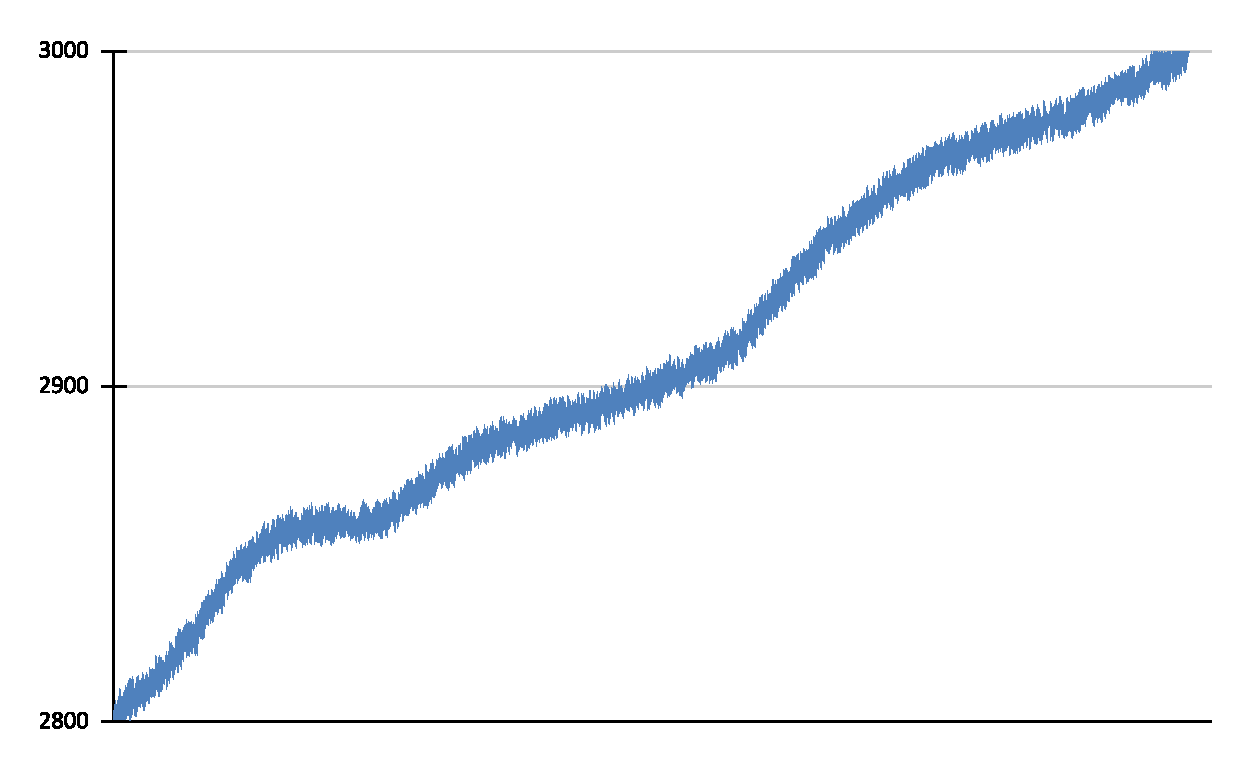
\includegraphics[width=\textwidth]{plc-orig.pdf}
        \caption{Naive Attack Reproduction}
        \label{fig:orig-attack}
    \end{subfigure}
    \hfill
    \begin{subfigure}[b]{0.49\textwidth}
        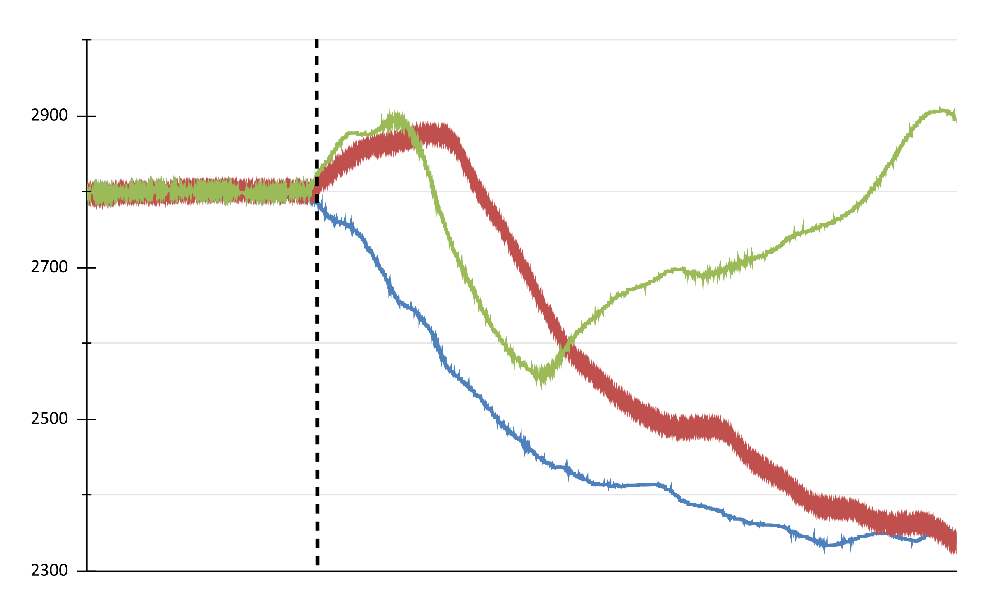
\includegraphics[width=\textwidth]{dashed-plc.pdf}
	    \caption{Voltage Corrected Destabilization}
        \label{fig:noconv-attack}
    \end{subfigure}
    \hfill
	\caption{\textbf{Left}: An attempt to stage the ICSREF attack using the recovered model without taking into account the physical effects of digital-to-analog conversion. \textbf{Right}: Variations of the staged attack with physical effects accounted for. The dashed line is the point at which the attack occurs (the 4 hour mark).}
    \label{fig:plc-eval}
\end{figure*}

Therefore, a naive digital twin of the firmware's implementation, maintaining the original voltage conversions, results in Fig.~\ref{fig:orig-attack} when staging the attack.
This is because, fundamentally, the input and output values to the PLC's equations are affected by the scaling decided by the physical digital-to-analog and analog-to-digital converters.
Code for this scaling does not exist in the firmware.
This proposes the importance of a hybrid approach to modeling in the current domain of firmware rehosting~\cite{jetset,p2im,halucinator}.
While an exact emulation of the firmware's operation is desirable for dynamic analysis and testing (e.g. fuzzing), it is also necessary to verify that the I/O boundaries of the system are consistent with the physical environment or environmental model the emulation is attached to.

Moving forward with this new understanding, we were able to correctly reproduce the destabilizing effects on reactor pressure created by uploading code to the PLC (Fig.~\ref{fig:noconv-attack}).
We corrected for the input value scaling in all cases, but we explore the effects of \emph{adding} semantics for the output scaling created by physical effects.
\textbf{Blue} represents the case where the output voltage is exactly matched to the inputs and outputs of Matlab. \textbf{Red} represents the case where the output voltage is modified to match the physical scaling created by the physical wiring of the PLC. \textbf{Green} represents the case where the attack \emph{did not} occur, and the output voltage scaling is applied to match the dynamics of the physical PLC.
These findings explain the otherwise unexplained ``bump'' in the graph of the original ICSREF paper, and demonstrate how InteGreat can be used to recover an abstract model of a program where no prior model exists.

\subsubsection{Discussion}

Informed by both the Jetset and \emph{Story Beyond the Eye} works, InteGreat adopts an opinionated perspective on the challenges facing binary program analysis.
It attempts to address universal and necessary limitations to abstract interpretation, such as the modeling of microarchitectural semantics and state explosion, by applying the well-worn technique of wrapping these complexities in a layer of abstraction (program slices), and then automates the construction of this abstraction.
While this alleviates the difficulties involved in inferring loop invariants and pointer analysis, InteGreat also has the explicit limitation of requiring users to leave these semantics undefined or provide their own formulae for resolution.

However, the abstraction of complex program semantics is also InteGreat's strength. 
By providing an interface for a more abstract representation the system during symbolic execution, InteGreat is able to rely on additional input for undefined or undecidable cases and extract useful models in cases where no such additional information is required or feasible to provide.
Moreover, by incorporating an object-oriented approach for abstraction specifications, the framework is also able to continually expand its base of knowledge.
The proposed dissertation will detail the trade-offs of abstraction and discuss the conditions under which InteGreat could be applied to the problems presented in Jetset and \emph{Story Beyond the Eye} thoroughly.



\section{Conclusion}

These three works, Jetset, \emph{Story Beyond the Eye}, and InteGreat, present three novel perspectives on the recovery of models from binary code.
In the first, the models were expression sets corresponding to the constraints of hardware peripheral interactions.
The second involved the more complex extraction and hand-modeling of glyph shifting schemes used to determine the information leaked by redacted text.
Finally, the third presented a more formal and sophisticated model for the extraction of meaningful abstractions from symbol-stripped, binary code.

As a whole, these works indicate a number of hard problems in the domain of binary program analysis, including the resolution and modeling of precise, discrete floating point operations and their relationship to the real domain, the ability to avoid difficulties incurred in developing a general solution to the halting problem through the use of abstraction, and the impossibility of perfectly rehosting a firmware image into an emulator and accurately interacting with it without \emph{some} knowledge of physical factors and additional hardware that plays a role in the system.

However, the resulting publications also make significant strides towards identifying the proper responses to each of these problems through the use of abstraction, careful evaluation of the algorithms under study, consideration of microarchitectural semantics, and novel binary analysis techniques.
The proposed dissertation will work to unify these findings and present them within a framework that is at once both detailed, empirically justified, clear, and unified.
It will also work to outline the core limitations of these works, and therefore provide useful commentary for future work in the domain of binary program analysis.

%%%%%%%%%%%%%%%%%%%%%%%%%%%%%%
% Section 4: Management Plan %
%%%%%%%%%%%%%%%%%%%%%%%%%%%%%%
\section{Time Line}

As the present author has present commitments for employment regardless of the outcome of his doctoral work, the dissertation will be subject to practical constraints on time in accordance with the current University of Illinois policies on dissertation timelines.
The absolute minimum time between the preliminary exam proposal and defense is four months, and the current scheduled date of the exam is February 24th.
As a result of aforementioned employment constraints, the present author intends to complete the writing of the defense by July 2023 and the proposed defense will occur at the end of this same month, the schedules of the defense committee permitting and considering all other university requirements have been fulfilled.

%%%%%%%%%%%%%%%%%%%%%%%%%%%%%%
% Section 5: Science Merit   %
%%%%%%%%%%%%%%%%%%%%%%%%%%%%%%
\section{Scientific Merit}



%%%%%%%%%%%%%%%%%%%%%%%%%%%%%%
% Section 6: Impact/Outreach %
%%%%%%%%%%%%%%%%%%%%%%%%%%%%%%

\section{Broader Impacts}
\label{broadimpacts}
\vspace*{-8pt}

This project will have direct impacts on research and education through access to simulation data products, student training, and K-12 outreach.  

\vspace{4pt}
\noindent \underline{\textit{Data Access}}: Maybe write about you will make data available.

\vspace{4pt}
\noindent \underline{\textit{Student Training}}: Write about how you will train students.

\vspace{4pt}
\noindent \underline{\textit{Some Other Outreach}}: Write about more outreach.

\vspace{4pt}
\noindent \underline{\textit{Dissemination}}: Write about how you will disseminate results (i.e., journal articles, workshops, etc).
\nocite*
